% !TeX root = ../main.tex
\chapter{Estado del arte}
\label{cap:estado-arte}
Este capítulo sitúa el proyecto en su contexto. En primer lugar se describe el simracing como disciplina y el uso que hacen del simulador pilotos, equipos, competiciones y aficionados (sección~\ref{sec:simracing-entrenamiento}). A continuación se exponen los fundamentos técnicos de los periféricos que componen un puesto de simulación (sección~\ref{sec:fundamentos-tecnicos}), y con ellos se analizan el mercado de periféricos, los productos comerciales y los proyectos abiertos existentes (sección~\ref{sec:productos-relacionados}). El capítulo termina identificando el hueco que pretende cubrir este trabajo (sección~\ref{sec:estado-arte-conclusion}).

\section{Simracing y entrenamiento en simuladores}
\label{sec:simracing-entrenamiento}

El simracing tiene su origen en los videojuegos de conducción, que nacieron casi al mismo tiempo que la propia industria del videojuego. En 1974, Atari lanzó \textit{Gran Trak~10}, considerado el primer videojuego de carreras de coches para máquinas recreativas. Ya incluía un volante, pedales de acelerador y freno y una palanca de cambios \parencite{wiki_grantrak10}, de modo que desde el principio el género buscó imitar los mandos de un coche real. Durante los años ochenta, las recreativas de carreras, como \textit{Pole Position} de Namco (1982), popularizaron el género. Su objetivo seguía siendo el entretenimiento, con un control sencillo y una física poco realista.

El paso del juego a la simulación llegó con el ordenador personal. En 1989, Papyrus Design Group publicó \textit{Indianapolis~500: The Simulation}, diseñado por David Kaemmer, que trataba de reproducir con fidelidad la carrera de Indianápolis. El juego permitía modificar los reglajes del coche y comprobar en tiempo real cómo cambiaba su comportamiento \parencite{wiki_indy500_sim}. Papyrus continuó esta línea con títulos como \textit{NASCAR Racing} y \textit{Grand Prix Legends} (1998), y buena parte de su equipo fundó después iRacing junto a John Henry, que lanzó su plataforma en 2008 \parencite{iracing_historia}.

En paralelo evolucionaron los periféricos. A finales de los noventa aparecieron los primeros volantes con \textit{force feedback} para PC, como el Microsoft SideWinder Force Feedback Wheel, presentado en 1998, que integraba un motor y un procesador propio para reproducir los baches, los golpes y las fuerzas en curva \parencite{microsoft_sidewinder_1998}. Desde entonces, simuladores y periféricos han avanzado de la mano: cada mejora en el modelo físico exige un hardware capaz de transmitirla y, a la vez, un hardware más preciso justifica simulaciones más detalladas. Esta evolución conjunta ha llevado al simracing desde el entretenimiento doméstico hasta las competiciones oficiales y el entrenamiento de pilotos profesionales, como se describe a continuación.

En esta sección estudiaremos este ecosistema, que es el simracing, y cómo lo emplean los diferentes tipos de usuarios.


\subsection{Simracing como disciplina}
\label{sec:simracing-mercado}

\paragraph{Definición.}
Se denomina \textit{simracing} (de \textit{simulated racing}) a la conducción de vehículos de competición en entornos virtuales tratando de representar con la mayor exactitud y fidelidad posible el comportamiento del vehículo y la representación del circuito o tramo en el que se compite. La evolución de este sistema depende tanto de la parte hardware que permite al usuario sentirse de la manera más próxima que está en el coche y depende también del apartado de software en el cual se incluye el videojuego o simulador que se va a tratar. Es importante diferenciar los diferentes tipos de videojuegos y qué es lo que ofrece al usuario final.

En un extremo están los juegos de tipo \textit{arcade}, que priorizan la diversión y la accesibilidad sobre el realismo. Su física se simplifica para que el coche sea fácil de controlar con un mando, y es habitual que incluyan elementos imposibles en la realidad, como turbos ilimitados o derrapes sin pérdida de velocidad. Es el caso de sagas como Mario Kart, Need for Speed o Forza Horizon \parencite{ruscio_2017_racing_realism}, pensadas para el ocio y no para reproducir la conducción real.


En el extremo opuesto tenemos los simuladores, que priorizan el realismo aunque eso haga que la conducción sea más difícil. Se modela en detalle el comportamiento del neumático, la transferencia de masas, la aerodinámica y la transmisión del vehículo, e incluso se pueden llegar a simular averías mecánicas o daños del coche. También se reproducen los circuitos con escaneos láser del trazado, llegando a obtener todos los detalles de la pista, como son baches, desperfectos del asfalto o incluso tramos de tierra; esto hace que la conducción sea mediante el uso de periféricos como volantes y pedales. En cuanto a simuladores, hay una variedad entre los que se encuentran iRacing, destacado por ser el simulador más realista y por su sistema competitivo online, y destinado a la competición de varias categorías de automovilismo licenciadas, como las 500~Millas de Indianápolis o las 24~Horas de Nürburgring; Assetto Corsa Competizione, destinado al mundial de GT; Assetto Corsa Rally, destinado a la simulación de rally, con recreaciones exactas de coches modernos y clásicos de toda la historia del rally, aunque actualmente está en desarrollo; Le Mans Ultimate, que simula el mundial de resistencia WEC y la IMSA, o Automobilista~2, que destaca por la simulación de vehículos históricos en circuitos tanto actuales como en variantes antiguas.


Por último, entre ambos extremos se encuentra lo que la comunidad denomina \textit{simcade}, que combina una física creíble con ayudas a la conducción y una presentación orientada al gran público. Estos títulos se pueden jugar con mando, pero admiten volante y pedales, y suelen ser la puerta de entrada al simracing. Pertenecen a esta categoría Gran Turismo~7, Forza Motorsport o la saga oficial de Fórmula~1 de EA Sports y Codemasters \parencite{ruscio_2017_racing_realism, kececi_2026_simracing_realism}. La frontera entre categorías no es rígida: Gran Turismo ha servido de base para la GT Academy y para competiciones oficiales, y el juego de Fórmula~1 es el que se usa en el campeonato de eSports de la propia categoría.

Como se ha expuesto, los simuladores de conducción han dejado de ser una herramienta usada exclusivamente por equipos de conducción para convertirse en un producto de consumo. Hoy en día, los simuladores son utilizados desde por pilotos profesionales, que estudian en profundidad el trazado de un circuito y sus características principales, además del propio comportamiento del vehículo, hasta por aficionados que compiten desde sus propias casas en ligas online o en torneos privados.

\paragraph{De entretenimiento a disciplina.}
La consolidación del simracing como algo más que un simple videojuego se apoya en una serie de hitos que se tratan más adelante en las siguientes subsecciones.
\begin{itemize}
	\item \textbf{2008, iRacing}. Nace el primer servicio de simulación por suscripción planteado como un deporte: licencias por categorías, índice de seguridad, calendario oficial y campeonatos con premios en metálico. Su base de usuarios pasó de unos 16\,000 suscriptores en su primer año a unos 50\,000 cinco años después.
	\item \textbf{2008, GT Academy}. Nissan y PlayStation lanzan un concurso para convertir a los jugadores más rápidos de Gran Turismo en pilotos reales. En la primera edición participaron unas 25\,000 personas y la ganó el español Lucas Ordóñez, que en 2011 terminó segundo de la clase LMP2 en las 24~Horas de Le~Mans \parencite{granturismo_web}. El programa demostró que las habilidades adquiridas en el simulador podían transferirse a la pista.
	\item \textbf{2017, F1 Esports Series}. La Fórmula~1 crea su campeonato oficial de simracing junto a Codemasters y Gfinity. Más de 60\,000 jugadores intentaron clasificarse en la primera edición, y a partir de 2018 los propios equipos de Fórmula~1 formaron sus equipos de eSports \parencite{formula1_news}.
	\item \textbf{2020, pandemia de COVID-19}. Con las competiciones reales suspendidas, el simracing ocupó su lugar. Pilotos en activo como Charles Leclerc, George Russell o Lando Norris corrieron los Virtual Grand Prix de la Fórmula~1, que sumaron unos 30~millones de visualizaciones entre televisión y plataformas digitales \parencite{formula1_news}, y iRacing pasó de unos 110\,000 a más de 160\,000 suscriptores activos en pocos meses \parencite{iracing_news}.
\end{itemize}
El resultado es que hoy el simracing tiene tres usos que conviven y se refuerzan entre sí: herramienta de entrenamiento y desarrollo para pilotos y equipos (secciones~\ref{sec:simracing-pilotos} y~\ref{sec:simracing-equipos}), competición con estructura deportiva propia (sección~\ref{sec:simracing-esports}) y afición (sección~\ref{sec:simracing-aficionados}).

La figura~\ref{fig:iracing-miembros} recoge los datos oficiales disponibles sobre los miembros de iRacing: un crecimiento sostenido durante la década de 2010 y un salto de más del 50\,\% en los primeros meses de la pandemia.

% Evolución de los miembros de iRacing (miles).
% Datos y fuentes:
%   jul 2012  35 000   iRacing, "iRacing Tops 35,000 Members"
%   sep 2014  52 000   iRacing, "A Billion Laps . . . and Counting!"
%   ene 2020 110 000   The Drive, citando al CFO Anthony Gardner (suscriptores activos)
%   abr 2020 160 000   The Drive, ídem
%   may 2020 170 000   iRacing, "iRacing Adds Multiple Servers..." (miembros activos)
\begin{figure}[htbp]
	\centering
	\begin{tikzpicture}
		\begin{axis}[
			grafica,
			xmin=2011.5, xmax=2021,
			ymin=0, ymax=190,
			clip=false,
			xtick={2012,2014,2016,2018,2020},
			xticklabel style={/pgf/number format/1000 sep={}},
			ylabel={Miembros (miles)},
		]
			\fill[serie2!12] (axis cs:2020.2,0) rectangle (axis cs:2021,190);
			\node[font=\footnotesize, text=tintasecundaria, anchor=south] at (axis cs:2020.6,190) {COVID-19};
			\addplot[serie1, line width=1.5pt, mark=*, mark size=2.5pt, mark options={fill=serie1, draw=white}]
				coordinates {
					(2012.54, 35) (2014.69, 52)
					(2020.04, 110) (2020.27, 160) (2020.34, 170)
				};
			\node[font=\footnotesize, anchor=south] at (axis cs:2012.54,37) {35\,000};
			\node[font=\footnotesize, anchor=south] at (axis cs:2014.69,54) {52\,000};
			\node[font=\footnotesize, anchor=east] at (axis cs:2019.95,110) {110\,000};
			\node[font=\footnotesize, anchor=east] at (axis cs:2020.15,170) {170\,000};
		\end{axis}
	\end{tikzpicture}
	\caption[Evolución de los miembros de iRacing]{Evolución de los miembros de iRacing entre 2012 y 2020. Los datos de 2012 y 2014 son miembros registrados y los de 2020, miembros activos. Fuente: comunicados de iRacing \parencite{iracing_news}.}
	\label{fig:iracing-miembros}
\end{figure}


\subsection{Pilotos profesionales}
\label{sec:simracing-pilotos}
En el ámbito profesional el simulador es una de las principales herramientas de entrenamiento del piloto. Conviven dos tipos: el simulador de ingeniería de los equipos, una instalación de gran tamaño gobernada por el modelo y los datos del coche real (sección~\ref{sec:simracing-equipos}), y el simulador personal que el piloto tiene en casa, construido con periféricos comerciales de gama alta. Esta subsección se centra en el segundo.

\paragraph{Usos del simulador.}
Los pilotos coinciden en tres usos. El primero es aprender o repasar circuitos: al estar escaneados con láser, permiten dar cientos de vueltas para fijar las referencias de frenada, los puntos técnicos del trazado o la entrada a boxes. El segundo es mantener el ritmo durante los parones de la temporada, cuando no pueden subirse al coche. El tercero es experimentar con el reglaje, como la carga aerodinámica o la altura, y comprobar su efecto sin arriesgar el coche real. A ellos se suma la competición virtual, que muchos disputan en campeonatos retransmitidos en directo. Hasta qué punto lo entrenado así sirve en la pista, y qué es lo que el simulador no puede reproducir, se analiza en la sección~\ref{sec:simracing-vida-real}.

\paragraph{Fórmula~1.}
La parrilla actual es la primera generación que ha crecido con el simulador como método de preparación. Lando Norris, campeón del mundo en 2025, lo usa desde las categorías de promoción y hoy entrena sobre todo en iRacing con un equipo de Cool Performance, la empresa de su hermano Oliver: habitáculo tipo Fórmula, pedales hidráulicos y base \textit{direct drive} de alta gama. La misma empresa ha equipado a otros pilotos, como Carlos Sainz, y Andrea Kimi Antonelli estrenó en 2026 un simulador a medida con el que prepara las carreras del calendario \parencite{gpfans_2026_antonelli}.

\paragraph{NASCAR.}
William Byron, piloto de Hendrick Motorsports en la NASCAR Cup Series, es un caso poco habitual de piloto formado en el simulador y no en el karting: empezó en iRacing con 13 años, ganó más de 100 carreras en 2012 y 2013 y, tras comprobar en Legends Cars que lo aprendido le servía en la pista, llegó a la Cup Series en 2018 con 20 años \parencite{motorsport_com}. Él mismo compara iRacing con un simulador de vuelo: una herramienta para perfeccionar habilidades, no un juego.

\paragraph{Resistencia.}
En la resistencia el simulador es a veces la única forma de rodar en un circuito. Más de la mitad del Circuito de la Sarthe, donde se disputan las 24~Horas de Le~Mans, son carreteras públicas que solo se cierran para la carrera, por lo que el Automobile Club de l'Ouest (ACO) obliga a todos los debutantes a superar una jornada de formación en simulador con tráfico, cambios de meteorología, conducción nocturna y zonas de velocidad limitada \parencite{fiawec_news}. Lo que se entrena no es tanto la vuelta rápida como la regularidad: mantener el ritmo en relevos largos y adelantar a coches más lentos de otras categorías sin perder tiempo.

La Nordschleife de Nürburgring, con más de 20~km y cerca de 170~curvas, muchas de ellas ciegas, plantea otro problema: exige cientos de vueltas para memorizarla, pero apenas hay días de entrenamiento y cada error se paga contra el guardarraíl. Tras el accidente mortal de 2015 en el Flugplatz \parencite{nls_news}, la federación alemana (DMSB) exige un permiso por niveles, el~B para iniciarse y el~A para los GT3 y las 24~Horas, del que ni Verstappen quedó exento \parencite{dmsb_permit_nordschleife, motorsport_com}. Desde la temporada 2025, terminar sin sanciones tres carreras de la NLS virtual sustituye en parte una de las carreras reales exigidas para el permiso~B \parencite{dmsb_permit_nordschleife}, lo que supone un reconocimiento oficial de que el simulador prepara para la pista.

Es también la disciplina en la que más se han mezclado la competición virtual y la real. En junio de 2020, con la carrera aplazada por la pandemia, el ACO y el WEC organizaron las primeras 24~Horas de Le~Mans Virtual, con 200 pilotos de 37~países, entre ellos Verstappen, Norris, Leclerc, Alonso o Button. El formato continúa como Le Mans Virtual Series, con equipos oficiales de Ferrari, Porsche o BMW, y desde 2024 el WEC tiene su simulador oficial, Le Mans Ultimate \parencite{fiawec_news}.

\paragraph{Rally.}
En el rally los tramos cambian de una temporada a otra, así que el simulador no sirve tanto para memorizar como para entrenar los reflejos del piloto y la lectura de notas con el copiloto. La referencia es Richard Burns Rally (2004), mantenido desde entonces por su comunidad y usado por pilotos del WRC y WRC2 como Craig Breen, Teemu Suninen o Nikolay Gryazin; la FIA ha empleado versiones modificadas para formar a sus delegados de seguridad. Kunos Simulazioni desarrolla ahora Assetto Corsa Rally con la intención de ocupar ese lugar \parencite{traxion_news}.

\paragraph{Max Verstappen.}
Entre los pilotos profesionales destaca Max Verstappen, cuatro veces campeón del mundo de Fórmula~1, para quien el simracing es una segunda actividad competitiva. Corre desde hace años con Team Redline, rebautizado en 2026 como Verstappen Sim Racing: ganó con Lando Norris las 24~Horas de Spa virtuales de 2019, y en 2024 su equipo se llevó las 24H de Daytona, Nürburgring y Spa. Las de Nürburgring las corrió desde un simulador que el equipo le instaló durante el fin de semana del Gran Premio de la Emilia Romaña, y ganó ambas carreras \parencite{traxion_news}. Su caso es, además, el ejemplo más claro de transferencia del simulador a una categoría distinta de la propia, como se ve en la sección~\ref{sec:simracing-vida-real}.

\subsection{Simulación en ámbito profesional}
\label{sec:simracing-equipos}
Además del simulador doméstico de los pilotos, existe un segundo nivel de simulación, el profesional. Equipos de competición, fabricantes de automóviles y academias de pilotos disponen de instalaciones propias, mucho más complejas, que forman parte de su proceso de trabajo y no solo de la preparación del piloto.

\paragraph{Equipos de competición.}
Los equipos de Fórmula~1 y de resistencia trabajan con simuladores de tipo \textit{driver-in-the-loop} (DIL): un monocasco real sobre una plataforma de movimiento, rodeado de una pantalla envolvente y
gobernado por el mismo modelo matemático del coche que usan los ingenieros. Su importancia creció a partir de 2009, cuando la Fórmula~1 prohibió los entrenamientos durante la temporada para reducir
costes \parencite{formula1_news}. Desde entonces los días en pista son muy escasos: en 2025 la pretemporada se redujo a tres días de pruebas y en 2026, con un reglamento técnico completamente nuevo, se amplió solo
a nueve \parencite{formula1_news}. Todo lo que no se puede probar en el circuito se prueba en el simulador.

Su uso se reparte a lo largo de todo el año. Antes de cada carrera, los pilotos y los pilotos de desarrollo ruedan en el simulador para preparar una base de reglajes y ensayar el circuito. Durante el fin de semana, mientras el equipo está en el circuito, la fábrica sigue trabajando: por la noche se
reproducen en el simulador los problemas detectados en los entrenamientos y se prueban soluciones que se aplican al día siguiente \parencite{mercedes_sim_driver}. Además, se usa para desarrollar el coche antes de que exista, evaluando nuevas piezas o configuraciones sin tener que fabricarlas. La inversión que exige
explica que los equipos renueven estas instalaciones como si fueran una pieza más del coche: Ferrari, por ejemplo, estrenó a finales de 2021 un nuevo simulador desarrollado por la empresa británica Dynisma para preparar el cambio de reglamento de 2022 \parencite{ferrari_2021_simulator}.

\paragraph{Fabricantes de automóviles.}
La simulación de conducción no se limita a la competición. Los fabricantes la utilizan para desarrollar sus coches de calle antes de construir prototipos. El caso más destacado es el Driving Simulation Centre de BMW en Múnich, terminado en 2020: ocupa 11\,400~m$^2$ y reúne 14~simuladores y
laboratorios, entre ellos uno con una zona de movimiento de casi 400~m$^2$ \parencite{bmw_2020_dsc}. En él se prueban sistemas de ayuda a la conducción, conducción autónoma, pantallas y mandos, e incluso la puesta a punto del chasis, con conductores reales, antes de pasar a la carretera \parencite{bmw_2020_dsc}.

La relación entre fabricantes y simracing funciona también en sentido inverso. Las marcas usan los simuladores de consumo como escaparate y como herramienta de trabajo para sus pilotos, como muestra el volante del BMW~M4~GT3 que Fanatec desarrolló con BMW M Motorsport y que se monta tanto en el coche real
como en el simulador (sección~\ref{sec:soluciones-comerciales}).

\paragraph{Academias y captación de talento.}
El simulador se ha convertido además en una vía de acceso a la competición. Tras la GT Academy de Nissan (sección~\ref{sec:simracing-mercado}), otros equipos crearon sus propios concursos. En 2017, McLaren organizó World's Fastest Gamer, al que se presentaron más de 30\,000 participantes. El ganador,
el neerlandés Rudy van Buren, superó una prueba final de cuatro horas en el simulador del equipo y obtuvo como premio un puesto de piloto de simulador oficial de McLaren para desarrollar el coche de 2018 \parencite{mclaren_2017_wfg}. El simulador sirve aquí como filtro de bajo coste: permite evaluar a miles de
candidatos sin necesidad de subirlos a un coche real.

En el otro extremo, el simulador también llega a la formación de conductores de calle. Endor, la empresa propietaria de Fanatec hasta 2024, comercializaba simuladores para autoescuelas en colaboración con una editorial especializada en formación vial \parencite{endor_web}.


\subsection{Del simulador a la vida real}
\label{sec:simracing-vida-real}
Los casos expuestos en las subsecciones anteriores plantean una pregunta: ¿qué parte de lo aprendido en el simulador sirve en la vida real? La experiencia de los pilotos y simracers permite responderla evaluando lo que sí es útil y las limitaciones del simulador.

\paragraph{Transferencia del simulador a la pista.}
Lo que mejor pasa del simulador a la pista es el conocimiento del circuito: las trazadas, los puntos de
frenada y las referencias visuales, que en los simuladores actuales coinciden con las reales gracias al
escaneo láser. También se transfieren el manejo del tráfico, la lectura de la carrera y los procedimientos, como las neutralizaciones o las paradas en boxes. Así lo muestran los pilotos de la sección~\ref{sec:simracing-pilotos}. William Byron comprobó en Legends Cars que lo aprendido en iRacing le servía en la pista. Louis Delétraz, ganador de las 24~Horas de Le~Mans Virtual de 2020 con Rebellion Williams Esport, debutó tres meses después en las reales y destacó lo parecidos que habían sido los kilómetros virtuales y los reales \parencite{fiawec_news}. Y Verstappen, que había preparado la Nordschleife durante años en el simulador, ganó en septiembre de 2025 su primera carrera de GT3 en la NLS y en mayo de 2026 lideró buena parte de las 24~Horas de Nürburgring hasta abandonar por la avería de un palier \parencite{nls_news, motorsport_com}. Lo confirman de forma todavía más clara los simracers que han dado el salto a la competición real:
\begin{itemize}
	\item \textbf{James Baldwin} ganó en 2019 la segunda edición de World's Fastest Gamer. Su única	experiencia real eran el karting y la Fórmula Ford, y apenas había probado el coche una vez antes de su debut. Aun así, en 2020 ganó su primera carrera del British GT con un McLaren~720S~GT3 \parencite{therace_2020_baldwin}.
	\item \textbf{Chris Lulham} se hizo profesional en iRacing en 2020 y ganó con Team Redline algunas de las grandes carreras virtuales, como las 24~Horas de Nürburgring y las 24~Horas de Le~Mans Virtual de
	2023. En 2025, ya en la competición real, ganó la Gold Cup del GT World Challenge Europe tanto en resistencia como en sprint, con una victoria de clase en las 24~Horas de Spa, y compartió con Verstappen la victoria en la NLS \parencite{traxion_news, nls_news}.
\end{itemize}
Ambos tenían experiencia previa en karting, lo que indica que el simulador no sustituye por completo la base de pilotaje real, pero sí acelera mucho el paso a categorías superiores.

\paragraph{Lo que no se transfiere.}
Los propios pilotos coinciden en que la principal diferencia es física. George Russell lo resume en dos ausencias: en el simulador no se siente la velocidad ni el miedo, porque un error se resuelve reiniciando la sesión, y tampoco se percibe el agarre de los neumáticos, que en el coche real se nota a
través del asiento \parencite{planetf1_russell_sim}. Verstappen añade un detalle técnico: en el simulador tiende a girar el volante de más, porque en el coche real nota cuándo se ha pasado y en la pantalla no \parencite{gpblog_verstappen_sim}. A ello se suma la exigencia física, ya que el simulador no reproduce las aceleraciones laterales y de frenada ni el calor del habitáculo, que en una carrera larga determinan el
rendimiento del piloto.

\paragraph{Implicaciones para los periféricos.}
Si el cuerpo del piloto no recibe las fuerzas del coche, toda la información que el simulador puede darle tiene que llegar a través de sus manos y sus pies. Por eso la calidad de la transferencia depende tanto del volante y los pedales. Una base con force feedback fiel permite notar la pérdida de
agarre que Russell echa en falta \parencite{toffin_2007_steering_feedback, murphy_2025_ffb_simracing}, y un freno que se dosifica por fuerza y no por recorrido reproduce el tacto del coche real. Preguntado por los periféricos que más importan, Verstappen respondió que, además de un buen ordenador, lo esencial es acertar con el pedal de freno y con la base del volante \parencite{caranddriver_verstappen_sim}, y él mismo ajusta su pedal de freno mucho más duro que la mayoría de los simracers precisamente porque así se parece más al de su coche \parencite{gpblog_verstappen_sim}. Estas dos
cuestiones, el force feedback y el freno por fuerza, son las que se desarrollan en los fundamentos técnicos de este capítulo (sección~\ref{sec:fundamentos-tecnicos}) y en el diseño de este trabajo.


\subsection{Competición y eSports}
\label{sec:simracing-esports}

El simracing tiene hoy una estructura competitiva propia, con campeonatos oficiales, equipos profesionales y premios en metálico. A diferencia de otros eSports, sus principales competiciones están organizadas o respaldadas por las propias categorías del automovilismo real.

\paragraph{Campeonatos oficiales.}
Las grandes categorías tienen su versión virtual. El campeonato de la Fórmula~1, que nació en 2017 como F1 Esports Series (sección~\ref{sec:simracing-mercado}), se disputa hoy como F1 Sim Racing World
Championship: en 2026 reúne a los equipos oficiales de Fórmula~1, con tres pilotos cada uno, en cuatro eventos y doce carreras, con 750\,000~dólares en premios \parencite{fanatec_web}. NASCAR organiza junto a iRacing la eNASCAR Coca-Cola iRacing Series, que en 2026 celebra su decimoséptima temporada con
500\,000~dólares en premios, 100\,000 de ellos para el campeón \parencite{iracing_news}. En resistencia, el ACO y el WEC organizan la Le Mans Virtual Series (sección~\ref{sec:simracing-pilotos}), y Gran Turismo
tiene su propio campeonato mundial, la Gran Turismo World Series, heredera de los campeonatos que organizaba con la FIA \parencite{granturismo_web}. Los fabricantes también organizan sus propias copas, como la Porsche Esports Supercup sobre iRacing \parencite{iracing_news}.

Su audiencia ha crecido con rapidez: la del campeonato de la Fórmula~1 en plataformas digitales se multiplicó por siete entre 2018 y 2021 (figura~\ref{fig:f1-esports-audiencia}).

% Audiencia en plataformas digitales del campeonato de eSports de la Fórmula 1 (millones de visualizaciones).
% Datos y fuentes:
%   2018   3,2   Formula 1, "F1 New Balance Esports Series 2018 watched by 4.4 million" (3,2 M en directo online; 1,2 M en TV aparte)
%   2019   5,8   Formula 1, "2019 F1 Esports Series records largest-ever audience" (audiencia online)
%   2020  11,4   Formula 1, "F1 Esports Series 2020 breaks viewing records..." (visualizaciones en directo, plataformas digitales)
%   2021  23,0   Traxion, "F1 Esports Series announces record-breaking 2021 viewing figures" (plataformas digitales)
\begin{figure}[htbp]
	\centering
	\begin{tikzpicture}
		\begin{axis}[
			grafica,
			ybar, bar width=26pt,
			ymin=0, ymax=26,
			xtick=data,
			xticklabel style={/pgf/number format/1000 sep={}},
			ylabel={Visualizaciones (millones)},
			nodes near coords,
			every node near coord/.append style={font=\footnotesize, text=black,
				/pgf/number format/fixed, /pgf/number format/precision=1},
			enlarge x limits=0.2,
		]
			\addplot[fill=serie1, draw=none]
				coordinates { (2018, 3.2) (2019, 5.8) (2020, 11.4) (2021, 23.0) };
		\end{axis}
	\end{tikzpicture}
	\caption[Audiencia digital del campeonato de eSports de la Fórmula 1]{Audiencia en plataformas digitales del campeonato de eSports de la Fórmula~1 entre 2018 y 2021. No incluye la audiencia televisiva ni los Virtual Grand Prix de 2020. Fuente: comunicados de la Fórmula~1 \parencite{formula1_news}.}
	\label{fig:f1-esports-audiencia}
\end{figure}


\paragraph{Equipos y patrocinio.}
Junto a los equipos de Fórmula~1 compiten estructuras profesionales dedicadas solo al simracing, como Team Redline, hoy Verstappen Sim Racing, que combinan simracers profesionales con pilotos reales. Su relación con los fabricantes de periféricos es estrecha: en el campeonato de Fórmula~1 todos los equipos usan material de Fanatec, socio oficial de la competición \parencite{fanatec_web}, y Simucube equipa a Verstappen Sim Racing (sección~\ref{sec:soluciones-comerciales}). Para estas marcas, las competiciones son el principal escaparate de su producto.

\paragraph{Límites del modelo.}
Pese a este crecimiento, el simracing sigue siendo un eSport minoritario fuera de su comunidad. En 2025 formó parte del Esports World Cup de Riad, el mayor torneo de videojuegos del mundo, pero su retransmisión registró la audiencia más baja de todo el evento, y en 2026 fue retirado del programa \parencite{traxion_news}. Las carreras de simulación son difíciles de seguir para quien no las practica, y el espectáculo depende en gran medida de la presencia de pilotos reales. El movimiento olímpico también lo ha incorporado de forma irregular: Gran Turismo formó parte de las Olympic Virtual Series de
2021, pero los primeros Juegos Olímpicos de eSports, previstos para 2027, están en suspenso \parencite{granturismo_web, pocketgamer_2025_olympic_esports}.

\subsection{Aficionados}
\label{sec:simracing-aficionados}

El aficionado es el usuario más numeroso del simracing y el destinatario de este trabajo. Su número ha crecido de forma sostenida desde la pandemia: solo iRacing supera los 300\,000 miembros activos \parencite{iracing_news} (figura~\ref{fig:iracing-miembros}), a los que se suman los usuarios de simuladores como Assetto Corsa Competizione, Le Mans Ultimate, Gran Turismo o la saga de Fórmula~1.

\paragraph{Cómo compite el aficionado.}
La mayoría de los aficionados compite en las carreras oficiales en línea de los simuladores, que los agrupan por nivel y por historial de seguridad, o en ligas organizadas por la propia comunidad, con
calendarios, reglamentos y comisarios propios. Algunos dan el salto a la competición real: los creadores de contenido Steve Alvarez Brown y Jimmy Broadbent, conocidos por sus canales de simracing, terminaron segundos de su clase en las 24~Horas de Nürburgring de 2025 con un BMW~M4~GT4 \parencite{blackfalcon_2025_n24}.

\paragraph{Una comunidad que crea contenido y hardware.}
El simracing ha generado además una comunidad muy activa en internet. Los canales dedicados a simracing superan el millón de suscriptores en YouTube, como Super GT, de Steve Alvarez Brown \parencite{alvarezbrown_supergt}, y pilotos como Norris o Verstappen retransmiten sus carreras en directo. Esa misma comunidad está detrás
de buena parte de los proyectos abiertos y de fabricación propia descritos en la sección~\ref{sec:soluciones-abiertas}: aficionados que, ante el precio de los periféricos comerciales, diseñan y comparten sus propias bases, pedaleras y botoneras.

\paragraph{La barrera del coste.}
El principal obstáculo para el aficionado es el precio del equipo. Como se verá en la sección~\ref{sec:mercado-perifericos}, la suscripción a un simulador cuesta unas decenas de euros, pero un puesto de gama media, con base \textit{direct drive}, aro y pedalera con célula de carga, supera con
facilidad los mil euros, sin contar el \textit{cockpit} ni el ordenador. Esa diferencia entre el coste del software y el del hardware deja un espacio para soluciones que acerquen las prestaciones de la gama media a un precio más bajo, que es el objetivo de este trabajo.


\section{Fundamentos técnicos de periféricos para simracing}
\label{sec:fundamentos-tecnicos}
Como se ha visto en la sección~\ref{sec:simracing-vida-real}, en el simulador no podemos experimentar las fuerzas y situaciones a las que se somete el piloto, por lo que necesitamos transmitir con la mayor precisión posible las sensaciones a través de la imagen, el audio y, lo que es más importante y en lo que se basa el proyecto, los periféricos: la transmisión de sensaciones mediante el volante y los pedales. Por esta misma razón, los periféricos cumplen una doble función. Deben recibir la información que transmite el simulador y enviar los cambios de estado a los periféricos, como puede ser el force feedback del volante, la iluminación de los LEDs del volante o la información que sale por pantalla en un dashboard; a esto se le denomina dispositivo de salida. Por otro lado, cumplen la función de enviar una señal para cambiar el estado actual, como al girar el volante, pisar un pedal o pulsar cualquier botón del volante o de una botonera; a esto se le denomina dispositivo de entrada.

Entre ambos sentidos se forma un lazo cerrado. El piloto actúa sobre los mandos, el simulador calcula la respuesta del coche a partir de esas entradas y devuelve al piloto las fuerzas y la información resultantes, que a su vez condicionan su siguiente acción. La calidad de la experiencia depende de que este lazo sea fiel y rápido: una medida imprecisa en la entrada o un retraso en la salida rompen la sensación de simulación.

La figura~\ref{fig:comunicacion-perifericos} resume este intercambio de información entre el piloto, los periféricos y el ordenador.

Esta sección describe los fundamentos técnicos de cada elemento de ese lazo, en el mismo orden en que la información lo recorre. Se empieza por el propio simulador y por la forma en que calcula y comunica las fuerzas a los periféricos (sección~\ref{sec:simulacion-conduccion}). A continuación se estudian las bases de \textit{force feedback} y sus tipos de transmisión (sección~\ref{sec:bases-ffb}), las pedaleras y los métodos para medir la entrada del piloto (sección~\ref{sec:pedaleras}) y los aros, que reúnen los mandos y la información que el piloto usa en pista (sección~\ref{sec:aros}). Por último se analiza el software de apoyo que completa el puesto (sección~\ref{sec:software-apoyo}). Estos fundamentos son los que se usan después como criterios para comparar los productos existentes (sección~\ref{sec:productos-relacionados}) y los que guían el diseño de este trabajo.

% Esquema de comunicación entre el piloto, los periféricos y el ordenador.
% Azul (serie1): entradas, del piloto al simulador. Naranja (serie2): salidas, del simulador a los periféricos.
% Gris: interacción física con el piloto. Coordenadas en cm; cada flecha tiene su propio carril para no cruzarse.
\begin{figure}[H]
	\centering
	\begin{tikzpicture}[
		font=\small,
		bloque/.style={draw=tintasecundaria, rounded corners=3pt, fill=white, align=center,
			minimum width=3.2cm, minimum height=1.1cm, inner sep=3pt},
		pc/.style={bloque, minimum height=2.0cm},
		grupo/.style={draw=tintasecundaria!55, dashed, rounded corners=6pt, inner sep=7pt},
		titulo/.style={font=\small\bfseries, text=tintasecundaria},
		entrada/.style={-{Stealth[length=2.4mm]}, line width=1.2pt, serie1},
		salida/.style={-{Stealth[length=2.4mm]}, line width=1.2pt, serie2},
		fisica/.style={-{Stealth[length=2.2mm]}, line width=0.9pt, tintasecundaria!85},
		etiqueta/.style={font=\scriptsize, inner sep=1.5pt, align=center},
	]
		% --- Bloques ---
		\node[bloque, minimum width=2.2cm, minimum height=5.6cm] (piloto) at (1.1,0.75)
			{\textbf{Piloto}\\[6pt] manos\\[2pt] pies\\[2pt] vista y oído};
		\node[bloque] (aro)      at (5.6, 3.0)  {\textbf{Aro}\\ botones, levas, LEDs};
		\node[bloque] (base)     at (5.6, 1.5)  {\textbf{Base \textit{direct drive}}\\ encoder y motor};
		\node[bloque] (pedalera) at (5.6, 0.0)  {\textbf{Pedalera}\\ sensores};
		\node[bloque] (dash)     at (5.6, -1.5) {\textbf{Dashboard}\\ pantalla};
		\node[pc]     (sim)      at (12.0, 1.5) {\textbf{Simulador}\\ modelo físico del\\ coche y la pista};
		\node[pc]     (apoyo)    at (12.0, -1.5) {\textbf{Software de apoyo}\\ dashes, LEDs};

		\begin{scope}[on background layer]
			\node[grupo, fit=(aro)(dash), label={[titulo]above:Periféricos}] (gperif) {};
			\node[grupo, fit=(sim)(apoyo), label={[titulo]above:Ordenador}] (gpc) {};
		\end{scope}

		% --- Interacción física (gris) ---
		\draw[fisica] (2.2, 3.0)  -- node[etiqueta, above] {girar,\\ pulsar} (aro.west);
		\draw[fisica] (base.west) -- node[etiqueta, above] {par en\\ las manos} (2.2, 1.5);
		\draw[fisica] (2.2, 0.0)  -- node[etiqueta, above] {pisar} (pedalera.west);
		\draw[fisica] (dash.west) -- node[etiqueta, above] {mirar} (2.2, -1.5);
		\draw[fisica, dashed] (gpc.south) -- (12.0, -3.05) -- node[etiqueta, above, pos=0.5] {imagen y sonido} (1.1, -3.05) -- (piloto.south);

		% --- Entradas (azul): periféricos -> simulador ---
		\draw[entrada] (7.2, 3.0)  -- (8.0, 3.0) -- (8.0, 2.35) -- node[etiqueta, above, pos=0.5] {USB HID:\\ ejes y botones} (10.4, 2.35);
		\draw[entrada] (7.2, 1.8)  -- (10.4, 1.8);
		\draw[entrada] (7.2, 0.0)  -- (8.0, 0.0) -- (8.0, 0.65) -- (10.4, 0.65);

		% --- Salidas (naranja): simulador -> periféricos ---
		\draw[salida] (10.4, 1.2) -- node[etiqueta, below, pos=0.5] {force feedback} (7.2, 1.2);
		\draw[salida] (sim.south) -- node[etiqueta, right] {telemetría} (apoyo.north);
		\draw[salida] (apoyo.west) -- node[etiqueta, above] {datos} (dash.east);
		\draw[salida] (13.6, -1.5) -- (14.3, -1.5) -- (14.3, 4.45) -- node[etiqueta, above, pos=0.5] {LEDs de revoluciones y avisos} (6.6, 4.45) -- (6.6, 3.55);

		% --- Leyenda ---
		\begin{scope}[shift={(2.6,-3.85)}, font=\scriptsize]
			\draw[entrada] (0,0) -- (0.6,0); \node[anchor=west] at (0.7,0) {entrada al simulador};
			\draw[salida]  (4.0,0) -- (4.6,0); \node[anchor=west] at (4.7,0) {salida hacia los periféricos};
			\draw[fisica]  (8.7,0) -- (9.3,0); \node[anchor=west] at (9.4,0) {interacción física};
		\end{scope}
	\end{tikzpicture}
	\caption[Comunicación entre el simulador y los periféricos]{Comunicación entre el piloto, los periféricos y el ordenador. Los periféricos envían al simulador la posición del volante, de los pedales y de los botones (entradas) y reciben de él el force feedback y los datos de telemetría que encienden los LEDs y el dashboard (salidas). (Fuente propia)}
	\label{fig:comunicacion-perifericos}
\end{figure}


\clearpage   % la subsección empieza en página nueva
\subsection{Simulación de conducción}
\label{sec:simulacion-conduccion}
El primer elemento de este lazo es el propio simulador, cuya función es calcular, a partir de las entradas del piloto, cómo se comporta el coche en cada instante y traducir dicho comportamiento en información que los periféricos puedan entender y reproducir. Para entender qué se le exige a una base o a una pedalera es necesario conocer antes qué calcula el simulador, con qué frecuencia lo hace y cómo se lo comunica al hardware.

\paragraph{Modelo físico del vehículo.}
El núcleo de un simulador es un modelo matemático que se resuelve de manera continua mientras el piloto conduce. Este modelo divide el vehículo en subsistemas intercomunicados entre sí: por un lado, el motor y la transmisión, que entregan el par a las ruedas; la suspensión, que reparte la carga entre las ruedas del vehículo y el comportamiento del mismo; la carga aerodinámica, la cual ejerce una fuerza vertical en función de la velocidad; y los neumáticos, que son los únicos puntos de apoyo del coche con la pista. Toda la fuerza que acelera, frena o hace girar el coche se genera en las cuatro pequeñas superficies en las que el neumático toca el suelo, por lo que el modelo de neumático es el componente que más diferencia a un simulador de otro. 

\subparagraph{Neumáticos.}
El comportamiento del neumático no tiene una forma lineal. La fuerza lateral que genera crece con el ángulo de deriva, es decir, la diferencia entre la dirección en la que apunta la rueda y la dirección en la que realmente se desplaza, hasta alcanzar un punto máximo donde el agarre del neumático disminuye y el coche desliza. Esta curva no solo depende del ángulo de deriva, sino de más factores como el empuje vertical generado por la carga aerodinámica, la temperatura, presión y desgaste. Para representarla, los simuladores emplean modelos empíricos, como la conocida \textit{fórmula mágica} de Pacejka \parencite{bakker_1987_tyre, pacejka_2012_tire}, o modelos físicos que simulan la deformación de la carcasa y de la banda de rodadura. La transferencia de masas completa el cuadro: al frenar la carga se desplaza hacia el eje delantero, al acelerar hacia el trasero y en curva hacia las ruedas exteriores, de modo que el agarre disponible en cada rueda cambia constantemente según lo que haga el piloto.

\begin{figure}[H]   % H: justo debajo del párrafo del neumático
	\centering
	\begin{minipage}[b]{0.30\textwidth}
		\centering
		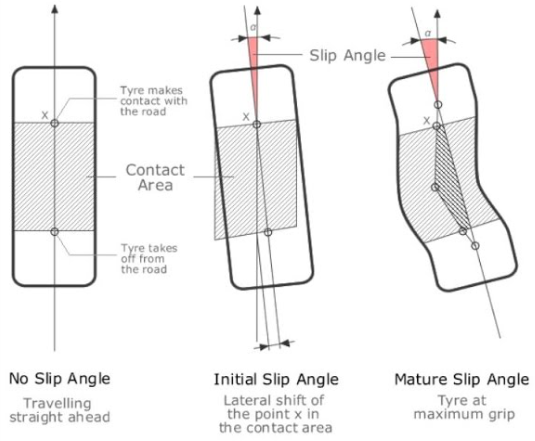
\includegraphics[width=\textwidth]{img/EA-angulo-deriva-neumatico.png}
		\caption{Deformación de la zona de contacto del neumático y ángulo de deriva~$\alpha$. Fuente: \parencite{iad_2026_deriva}.}
		\label{fig:angulo-deriva}
	\end{minipage}
	\hspace{0.05\textwidth}
	\begin{minipage}[b]{0.50\textwidth}
		\centering
		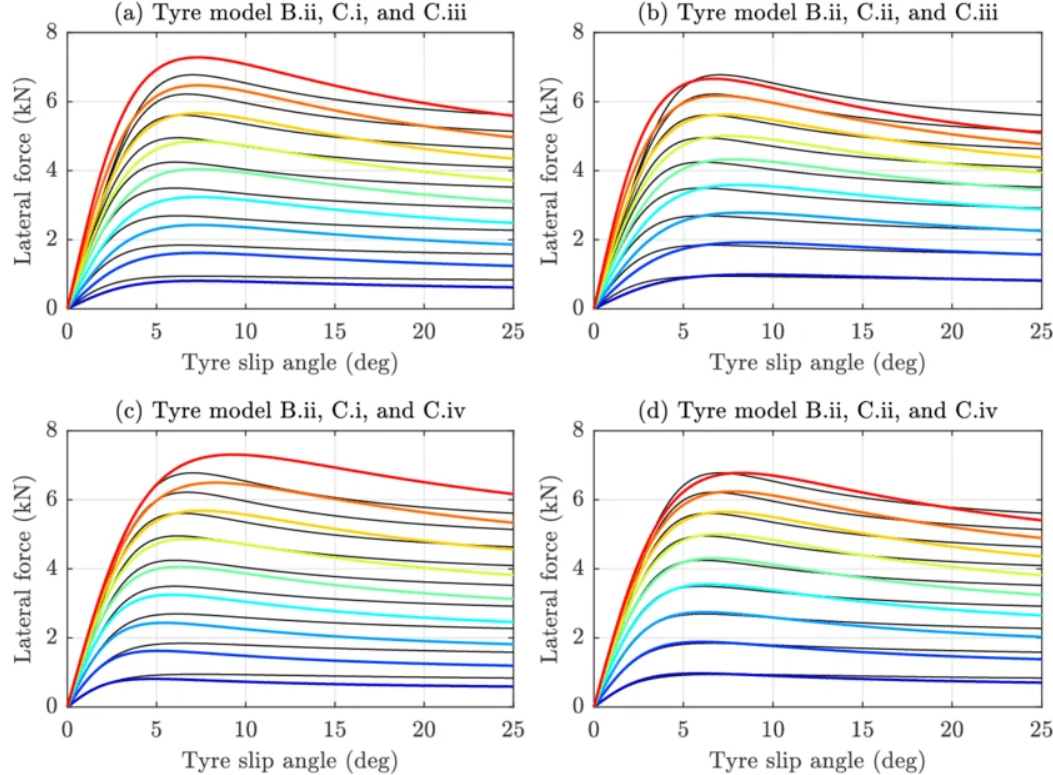
\includegraphics[width=\textwidth]{img/EA-formula-magica-neumatico.png}
		\caption{Fuerza lateral del neumático en función del ángulo de deriva para distintas cargas verticales (en color, modelos; en negro, datos medidos). Fuente: \parencite{sciencedirect_magic_formula}.}
		\label{fig:formula-magica}
	\end{minipage}
\end{figure}

\subparagraph{Vehículo.}
El resto del vehículo se divide en subsistemas: el motor y la transmisión, que entregan el par a las ruedas; la suspensión, que reparte las cargas entre ellas; la aerodinámica, que añade carga vertical en función de la velocidad; y los frenos. La transferencia de masas los relaciona entre sí: al frenar la carga se desplaza hacia el eje delantero, al acelerar hacia el trasero y en curva hacia las ruedas exteriores, de modo que el agarre disponible en cada neumático cambia constantemente según lo que haga el piloto.

Para que este modelo sea fiel, los desarrolladores trabajan con datos de coches reales, como planos CAD, medidas de suspensión, curvas de motor y datos aerodinámicos proporcionados por los fabricantes y equipos, además de cómo se comportan las ayudas electrónicas; estos datos son validados por pilotos que conducen dichos coches. Sobre este modelo se pueden modificar parámetros del vehículo para mejorar su rendimiento en los diferentes circuitos: altura y dureza de la suspensión, estabilizadores, ángulo de los alerones, presión de los neumáticos, relaciones de las marchas de la caja de cambios y reparto de frenada entre ejes. Cada cambio altera la física del coche y, con ella, su comportamiento y las fuerzas que llegan al volante.

Los simuladores más completos modelan además los daños y el desgaste mecánico. Un golpe puede deformar la suspensión o romper el alerón y desequilibrar el coche, los frenos pierden eficacia al sobrecalentarse y el motor o la caja de cambios pueden averiarse por un uso inadecuado.

Las figuras~\ref{fig:telemetria-motor} y~\ref{fig:telemetria-suspension} muestran algunas de estas magnitudes registradas durante una vuelta en el simulador.

\begin{figure}[H]   % H: justo aquí, debajo del subpárrafo «Vehículo»
	\centering
	% Mismo alto en las dos imágenes; el ancho de cada columna sigue la proporción de su captura
	\begin{minipage}[t]{0.478\textwidth}
		\centering
		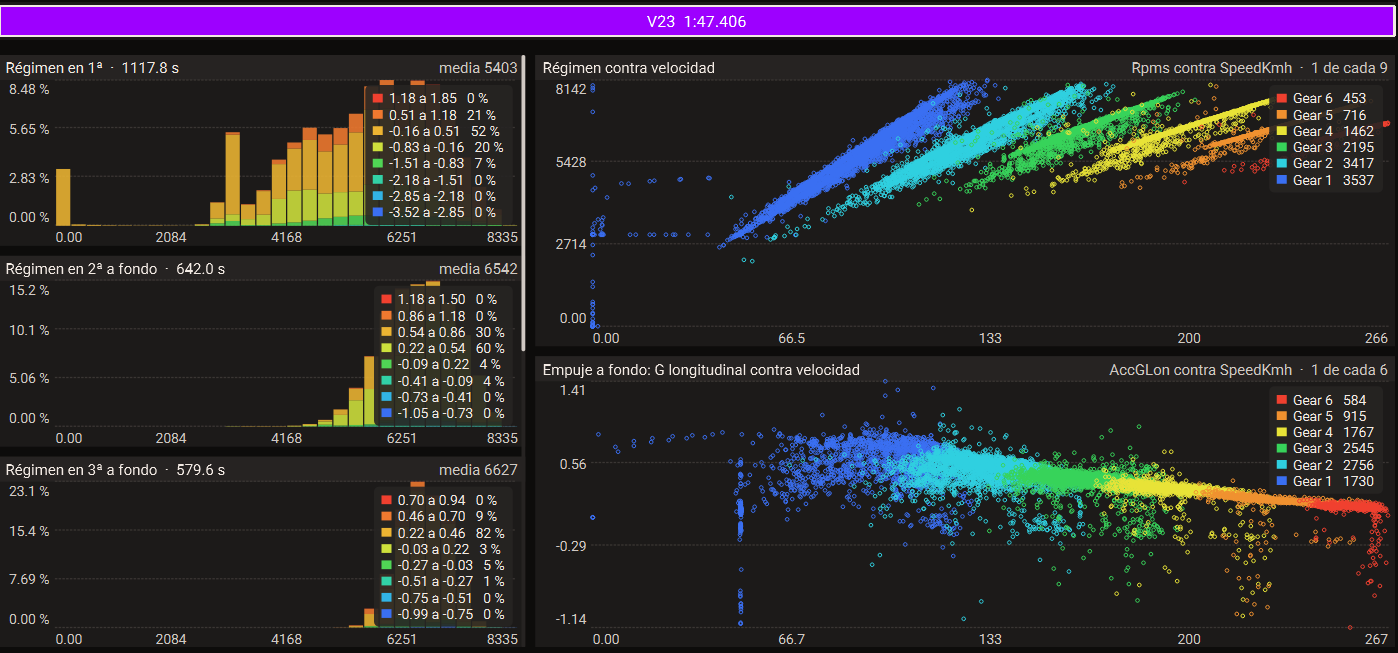
\includegraphics[width=\linewidth]{img/EA-rpmHisto.png}
		\caption[Telemetría del motor y la transmisión en una vuelta de simulador]{Motor y transmisión en una vuelta de 1:47,406. A la izquierda, el régimen en primera, segunda y tercera; a la derecha, régimen y aceleración longitudinal frente a la velocidad, un color por marcha: cada marcha forma su propia recta y muestra el escalonamiento de la caja de cambios.}
		\label{fig:telemetria-motor}
	\end{minipage}
	\hfill
	\begin{minipage}[t]{0.502\textwidth}
		\centering
		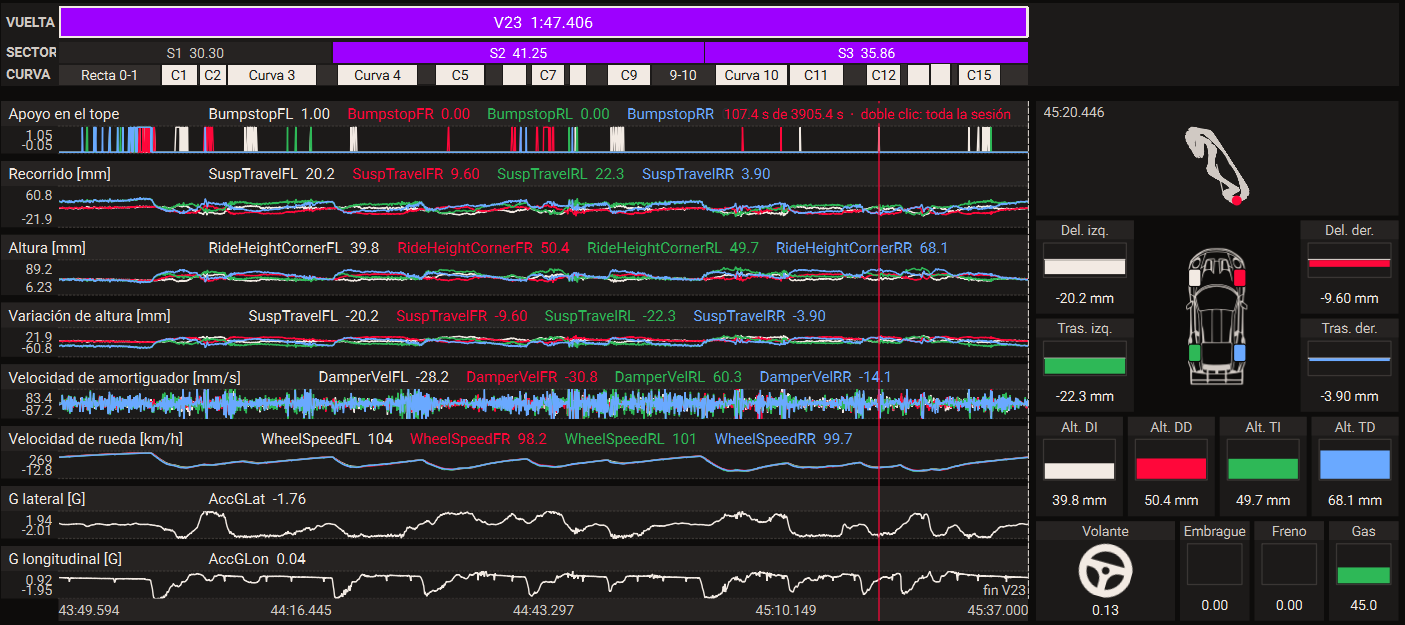
\includegraphics[width=\linewidth]{img/EA-suspensionHisto.png}
		\caption[Telemetría de la suspensión en una vuelta de simulador]{Suspensión en la misma vuelta, por sectores y curvas: tope, recorrido y altura de cada rueda, velocidad de los amortiguadores y de las ruedas, y aceleraciones lateral y longitudinal.}
		\label{fig:telemetria-suspension}
	\end{minipage}
	\par\medskip
	{\footnotesize Fuente de ambas figuras: capturas del analizador de telemetría del Configurador de VH SimGrid.}
\end{figure}

\subparagraph{Circuito.}
El modelo del coche se apoya en un modelo igual de detallado del circuito. Como se ha visto en la sección~\ref{sec:simracing-mercado}, los simuladores actuales reproducen los trazados a partir de escaneos láser del circuito real, con una precisión de milímetros que recoge los baches, los cambios de rasante, las variaciones de adherencia del asfalto y la forma exacta de los pianos. Estos detalles no son solo visuales: cada irregularidad de la superficie altera la carga de los neumáticos y, por tanto, las fuerzas que el piloto debe percibir a través del volante.

\paragraph{Frecuencia de cálculo y envío de datos.}
El modelo físico se resuelve en pasos discretos de tiempo, y la frecuencia con la que se hace condiciona la información que llega al piloto. Es importante diferenciar la frecuencia interna de la física y la frecuencia con la que el simulador envía la consigna a la base, que no coinciden siempre. iRacing es el caso más documentado: su física se resuelve internamente a 360~Hz, pero el cálculo del \textit{force feedback} y su envío al volante se hacen a 60~Hz, por lo que la base recibe un valor nuevo cada 16,7~ms \parencite{iracing_360hz}. Desde 2024 el simulador ofrece un modo de 360~Hz para las bases compatibles: en cada envío de 60~Hz incluye seis muestras, y es el firmware de la base el que las reproduce de forma escalonada. Este modo transmite señales de mayor frecuencia, como el golpe de un piano, a cambio de añadir un retraso de unos 16~ms \parencite{iracing_360hz}. rFactor~2, en cambio, lee la posición del volante y actualiza la salida de \textit{force feedback} a 400~Hz \parencite{overtake_ffb_analysis}.

Una frecuencia más alta no garantiza por sí sola una mejor sensación. Si el modelo físico completo no se calcula a esa velocidad, el simulador se limita a interpolar valores intermedios, y un modelo de neumático pobre no mejora por enviarse más a menudo \parencite{simxperience_ffb_myths}. Lo que sí se deduce de estas cifras es que la base debe trabajar a una frecuencia muy superior a la del simulador: entre dos consignas consecutivas tiene que mantener el par, suavizar la transición y responder por sí misma a los movimientos del piloto. Esta tarea, que se trata en la sección~\ref{sec:bases-ffb}, corresponde al firmware de la base y no al simulador.

\paragraph{Comunicación con los periféricos.}
En el ordenador, los periféricos de simracing se presentan como dispositivos USB de clase HID (\textit{Human Interface Device}), la misma que usan teclados, ratones y mandos. Esta clase permite al ordenador detectar estos dispositivos sin necesidad de controladores específicos: cada dispositivo describe en un descriptor qué ejes, botones y otros controles tiene, y el simulador los lee como si fueran un joystick. Las pedaleras, los aros y las botoneras se limitan a este papel de entrada y envían periódicamente la posición de sus ejes y el estado de sus botones.

Las bases, como se comentó anteriormente, no se limitan a enviar la posición actual del volante: también reciben información. Para ello la especificación HID incluye una extensión, la clase PID (\textit{Physical Interface Device}), que define cómo un programa  puede crear, modificar, iniciar y detener efectos de fuerza en un dispositivo \parencite{usb_hid_pid}. En Windows, los simuladores acceden a esta funcionalidad a través de la interfaz DirectInput, que agrupa los efectos en tres familias  \parencite{simracingcockpit_ffb}:
\begin{itemize}
	\item \textbf{Fuerza constante}: un par de valor y sentido determinados, que se actualiza cada vez que el simulador envía una nueva consigna. Es el efecto que usan los simuladores para transmitir la fuerza calculada en la dirección, y en la práctica el más importante.
	\item \textbf{Efectos periódicos}: señales con forma de onda (senoidal, cuadrada, triangular o diente de sierra) de amplitud y frecuencia configurables, que se emplean para vibraciones como las del motor o las de un piano.
	\item \textbf{Efectos condicionales}: fuerzas que dependen del estado del propio volante, como el muelle (proporcional al ángulo de giro), el amortiguador (proporcional a la velocidad), la fricción y la inercia (proporcional a la aceleración).
\end{itemize}

La diferencia entre las familias es relevante para el diseño de una base. La fuerza constante la calcula el simulador y la base solo tiene que reproducirla. Los efectos periódicos y condicionales, en cambio, se envían una sola vez con sus parámetros y es el firmware de la base el que los genera, leyendo su propio encoder a alta frecuencia. Una base compatible con el estándar debe implementar todos ellos, porque cada simulador usa una combinación distinta. Este es precisamente el papel de la capa de efectos HID de OpenFFBoard descrita en la sección~\ref{sec:soluciones-abiertas}.  

\paragraph{Telemetría.}
Los simuladores publican en tiempo real el estado completo de la sesión, como las revoluciones por minuto del motor, velocidad, estado de las suspensiones, tiempos por vuelta, temperatura y presión de los neumáticos, posición actual del piloto en la sesión y un largo conjunto de datos que cada simulador publica. Estos datos no se envían a los periféricos por la vía HID, sino que se ponen a disposición de otros programas del mismo ordenador. Los métodos más habituales son mediante memoria compartida y mediante el protocolo de comunicación UDP: Assetto Corsa Competizione, por ejemplo, usa la primera y la saga de Fórmula~1 de EA, la segunda \parencite{kunos_acc_shared_memory, ea_f1_25_udp}.

La telemetría es la fuente de información de todo lo que se muestra al piloto aparte del par en el volante como los LEDs, los \textit{dashes} con los datos del coche, los avisos de un ingeniero por voz o el análisis de las vueltas una vez terminada la sesión. Cada simulador la expone con un formato propio, por lo que cualquier programa que quiera usarla debe adaptarse a cada uno. Este problema, y las herramientas que lo resuelven, se tratan en la sección~\ref{sec:software-apoyo}.

\paragraph{Implicaciones para los periféricos.}
De lo anterior se desprenden los requisitos que el simulador impone al hardware. La base debe aceptar consignas de par por el protocolo HID PID, implementar los efectos estándar y trabajar a una frecuencia muy superior a la del simulador para reproducir la fuerza sin retrasos ni escalones. Los periféricos de entrada deben medir con suficiente resolución y frecuencia para que el modelo físico reciba las acciones del piloto tal como se producen. Y el conjunto debe poder aprovechar la telemetría para devolver al piloto la información que el par no transmite. Las siguientes subsecciones estudian cómo resuelve cada periférico estos requisitos.

\subsection{Bases de force feedback}
\label{sec:bases-ffb}

La base es el dispositivo que cierra el lazo en el sentido de la salida. Recibe del simulador la consigna del par calculada en la dirección del coche (sección~\ref{sec:simulacion-conduccion}) y la convierte en un par real en el eje del volante, que el piloto nota en las manos. Al mismo tiempo mide el ángulo de giro y lo devuelve al simulador como entrada. Todas las bases se componen de los mismos elementos: un motor eléctrico que genera el par, la transmisión que lo lleva hasta el eje, un sensor que mide la posición, una fuente de alimentación y un firmware que coordina el conjunto. Lo que diferencia una base de entrada de una profesional es cómo se resuelve cada uno de ellos.

\paragraph{Tipo de transmisión.}
La transmisión es el elemento que más condiciona el tacto de la base, y es el criterio con el que el mercado clasifica sus productos (sección~\ref{sec:mercado-perifericos}). Existen tres soluciones.

\subparagraph{Engranajes.}
Un motor de corriente continua pequeño y rápido mueve el eje del volante a través de un tren de engranajes que multiplica su par. Es la solución más barata y la de los volantes de entrada, como el Logitech~G29, que alcanza unos 2,2~N\,m \parencite{logitech_g29}. Sus inconvenientes son mecánicos. La holgura entre los dientes (\textit{backlash}) crea una pequeña zona muerta en la que el volante gira sin oponer resistencia, precisamente alrededor del centro, que es donde el piloto necesita más precisión. El paso de un diente a otro produce además un rizado que se nota como una textura granulosa, y el engranaje es ruidoso. Para disimular estos defectos, los fabricantes filtran la señal de \textit{force feedback}, y con ello se pierden los detalles más finos.

\subparagraph{Correa.}
El motor mueve el eje mediante una o varias correas dentadas y poleas de distinto diámetro. La correa elimina la holgura y el rizado de los engranajes, de modo que el tacto es mucho más suave y silencioso, y permite usar motores mayores, con pares de entre 4 y 8~N\,m. A cambio, la correa es elástica: se estira ligeramente bajo carga, lo que introduce un pequeño retraso y amortigua los cambios bruscos de fuerza. Además, el rozamiento de las poleas y la inercia del conjunto se suman a los del propio volante. Esta solución dominó la gama media antes de la llegada del \textit{direct drive}, y algunas bases combinan correa y engranajes en una transmisión híbrida, como el Thrustmaster~T150 \parencite{bsimracing_2015_t150}.

\subparagraph{Accionamiento directo (\textit{direct drive}).}
El volante se monta directamente sobre el eje del motor, sin ninguna reducción intermedia. Al no haber transmisión, desaparecen la holgura, el rizado, la elasticidad y el rozamiento añadidos: el par que genera el motor es exactamente el que llega a las manos del piloto, y cualquier detalle de la señal, por pequeño o rápido que sea, se transmite sin pérdidas. El precio de esta simplicidad es que el motor debe generar por sí solo todo el par, sin la multiplicación de una reducción. Por eso las bases \textit{direct drive} usan motores grandes y de alto par a baja velocidad, y necesitan una electrónica de control mucho más exigente. Hasta hace pocos años esto las limitaba a la gama profesional, pero hoy, como se ha visto, ofrecen desde unos 4~N\,m en la gama de entrada hasta 35~N\,m en la profesional \parencite{moza_web, simucube_web}.

La tabla~\ref{tab:transmisiones} resume las diferencias entre las tres soluciones.

\begin{table}[htbp]
	\centering
	\caption[Comparación de los tipos de transmisión de las bases de \textit{force feedback}]{Comparación de los tipos de transmisión de las bases de \textit{force feedback}. Adaptado de: \parencite{logitech_g29, moza_web, simucube_web}}
	\label{tab:transmisiones}
	\small
	\begin{tabular}{|l|c|c|c|}
		\hline
		\textbf{Característica} & \textbf{Engranajes} & \textbf{Correa} & \textbf{Direct drive} \\
		\hline
		Par típico (N\,m)       & 2--3       & 4--8       & 4--35 \\
		Holgura central         & Sí         & No         & No \\
		Rizado mecánico         & Alto       & Bajo       & Nulo \\
		Elasticidad / retraso   & Bajo       & Medio      & Nulo \\
		Ruido                   & Alto       & Bajo       & Muy bajo \\
		Detalle transmitido     & Bajo       & Medio      & Alto \\
		Coste                   & Bajo       & Medio      & Medio--alto \\
		\hline
	\end{tabular}
\end{table}

\paragraph{Motor.}
Las bases de engranajes y de correa usan motores de corriente continua con escobillas, sencillos de controlar: el par es proporcional a la corriente que circula por ellos, y basta con regular esa corriente. Las escobillas, sin embargo, se desgastan, producen rozamiento y limitan el par que el motor puede mantener.

Las bases \textit{direct drive} emplean motores síncronos de imanes permanentes sin escobillas, conocidos como  BLDC (\textit{Brushless DC}) o PMSM (\textit{Permanent Magnet Synchronous Motor}) según la forma de su fuerza contraelectromotriz \parencite{krishnan_2010_pmsm}. En ellos los imanes están en el rotor y los devanados en el estátor, de modo que no hay contactos que se desgasten y el calor se genera en la parte fija, donde es más fácil disiparlo. Para obtener mucho par a baja velocidad se usan motores de gran diámetro y muchos pares de polos, con una construcción similar a la de los motores de buje de bicicletas y patinetes eléctricos. Esta semejanza es la que aprovechan los proyectos de fabricación propia, y también este trabajo, para construir bases \textit{direct drive} a bajo coste.

Un defecto propio de estos motores es el \textit{cogging}: la atracción entre los imanes del rotor y los dientes del estátor crea unas posiciones preferentes en las que el rotor tiende a quedarse, y que se notan como pequeños escalones al girar el volante con la base sin par. Los fabricantes lo reducen con el diseño del motor, inclinando los imanes o las ranuras, o lo compensan desde el firmware midiendo su forma y aplicando un par opuesto \parencite{bianchi_2002_cogging, jahns_1996_torque_ripple, petrovic_2000_torque_ripple}.

\begin{figure}[htbp]
	\centering
	\captionsetup{justification=raggedright, singlelinecheck=false}   % columnas estrechas: pies sin justificar
	\begin{minipage}[b]{0.32\textwidth}
		\centering
		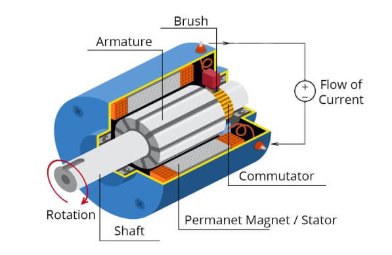
\includegraphics[width=\textwidth]{img/EA-motorDC.png}
		\caption[Motor de corriente continua con escobillas]{Motor de corriente continua con escobillas. Fuente: \parencite{salim_2025_brushed_dc}}
		\label{fig:motor-escobillas}
	\end{minipage}
	\hfill
	\begin{minipage}[b]{0.32\textwidth}
		\centering
		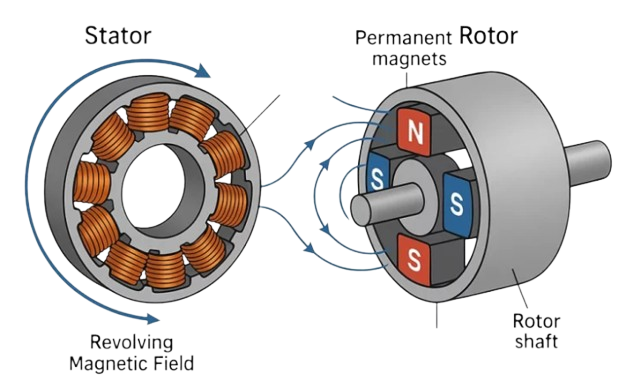
\includegraphics[width=\textwidth]{img/EA-motorBLDC.png}
		\caption[Motor sin escobillas de imanes permanentes (BLDC/PMSM)]{Motor sin escobillas de imanes permanentes (BLDC/PMSM). Fuente: \parencite{krishnan_2010_pmsm}}
		\label{fig:motor-bldc}
	\end{minipage}
	\hfill
	\begin{minipage}[b]{0.32\textwidth}
		\centering
		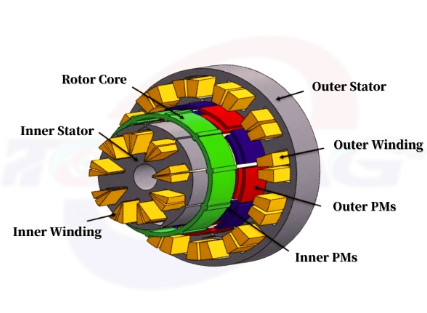
\includegraphics[width=\textwidth]{img/EA-motorPMSM.png}
		\caption[Motor de imanes permanentes de doble estátor]{Motor de imanes permanentes de doble estátor. Fuente: \parencite{wang_2011_double_stator}}
		\label{fig:motor-doble-estator}
	\end{minipage}
\end{figure}

\paragraph{El control vectorial (FOC).}
A diferencia del motor con escobillas, en un motor sin escobillas la corriente de cada fase debe conmutarse electrónicamente según la posición del rotor. La técnica que se usa en las bases de calidad es el control orientado al campo (\textit{Field Oriented Control}, FOC), también llamado control vectorial \parencite{krishnan_2010_pmsm}. Su idea es transformar las tres corrientes de fase, que son senoidales y dependen del ángulo del rotor, en dos componentes constantes referidas al propio rotor:
\begin{itemize}
	\item La corriente $i_q$ (en cuadratura), perpendicular al campo de los imanes, que es la que produce el par.
	\item La corriente $i_d$ (directa), alineada con el campo, que no produce par y que normalmente se mantiene en cero.
\end{itemize}
Este cambio de referencia se hace con dos transformaciones matemáticas, la de Clarke, que pasa de las tres fases a un sistema de dos ejes fijos, y la de Park, que gira ese sistema con el rotor usando el ángulo medido por el encoder. En el sistema resultante, el motor sin escobillas se comporta como uno de corriente continua, y el par es directamente proporcional a una sola corriente:
\begin{equation}
	T = k_t \, i_q
	\label{eq:par-foc}
\end{equation}
donde $k_t$ es la constante de par del motor, en N\,m/A. De este modo, convertir la consigna del simulador en par se reduce a controlar $i_q$ mediante un regulador PI, que compara la corriente medida con la deseada y ajusta la tensión aplicada a cada fase mediante modulación por ancho de pulso (PWM). Este lazo de corriente se ejecuta a varias decenas de kilohercios, cientos de veces más rápido que la consigna del simulador, y es el que garantiza que el par llega al volante sin rizado y sin retraso apreciable \parencite{briz_2000_current_regulators}. La ecuación~\ref{eq:par-foc} explica también por qué el FOC es imprescindible en el \textit{direct drive}: como no hay reducción que filtre las imperfecciones, cualquier error en el control de la corriente se nota directamente en las manos del piloto.

\paragraph{Medida de la posición.}
La base necesita conocer el ángulo del eje por dos motivos: el control FOC lo usa para orientar las corrientes en cada ciclo, y el simulador lo recibe como la posición del volante. Para ello se emplea un encoder, que puede ser de dos tipos según la tecnología:
\begin{itemize}
	\item \textbf{Ópticos}: un disco con ranuras gira entre un emisor de luz y un receptor, y cada ranura que pasa genera un pulso. Ofrecen alta resolución y no les afectan los campos magnéticos del motor.
	\item \textbf{Magnéticos}: un sensor mide la orientación de un imán solidario al eje. Son más baratos y compactos, pero su precisión depende de la alineación y pueden verse afectados por el campo del motor.
\end{itemize}
Además, el encoder puede ser incremental, que solo cuenta pulsos desde el arranque y necesita una referencia para conocer el centro, o absoluto, que conoce su posición en cuanto recibe alimentación. Su resolución determina la precisión con la que se mide el volante y la suavidad del control: en una base \textit{direct drive}, donde el giro del volante coincide con el del motor, un encoder de baja resolución se nota como pequeños escalones en el par.

\paragraph{Parámetros de una base.}
Más allá del tipo de transmisión, hay varios parámetros que definen las prestaciones de una base:
\begin{itemize}
	\item \textbf{Par máximo}: el par más alto que puede aplicar. Conviene distinguir entre el par de pico, que solo se mantiene unos instantes, y el par sostenido, que el motor aguanta sin sobrecalentarse. Un par elevado no se usa para que el volante sea más duro, sino para tener margen y reproducir sin saturar los golpes y los picos de fuerza.
	\item \textbf{Velocidad de respuesta} (\textit{slew rate}): la rapidez con la que el par puede cambiar, en N\,m/ms. Determina si la base reproduce fielmente los cambios bruscos, como un piano o una pérdida repentina de agarre.
	\item \textbf{Frecuencia de control}: la frecuencia del lazo de corriente y del procesamiento de efectos. Debe ser muy superior a la de la consigna del simulador para que la base pueda interpolar entre muestras y responder a los movimientos del piloto (sección~\ref{sec:simulacion-conduccion}).
	\item \textbf{Resolución del encoder}: cuentas por vuelta del sensor de posición.
	\item \textbf{Inercia y rozamiento propios}: los que añaden el rotor y la transmisión, que el piloto nota como un volante más pesado o más perezoso de lo que debería.
\end{itemize}

\paragraph{El firmware de la base.}
Entre la consigna del simulador y el lazo de corriente se sitúa el firmware de la base, que tiene tres funciones. La primera es atender la comunicación USB: presentarse como dispositivo HID, enviar el ángulo del volante e interpretar los efectos HID PID descritos en la sección~\ref{sec:simulacion-conduccion}, generando por sí mismo los efectos periódicos y condicionales.

La segunda es acondicionar la señal. Como la consigna llega a una frecuencia baja y en escalones, el firmware aplica un filtro de reconstrucción que suaviza la transición entre muestras. Además añade efectos propios que el usuario ajusta según su gusto: amortiguación, fricción e inercia simuladas, que dan cuerpo al volante y evitan oscilaciones, y limitadores de velocidad y de par. Estos ajustes son los que cada fabricante expone en su aplicación de configuración (sección~\ref{sec:soluciones-comerciales}).

La tercera es la seguridad. Una base \textit{direct drive} de gama media puede generar un par suficiente para lesionar la muñeca o el pulgar del piloto si el volante gira bruscamente, por ejemplo tras un choque en el simulador o por un error de comunicación. Por ello el firmware limita el par y la velocidad, corta la potencia si pierde la conexión con el ordenador, y las bases incluyen un pulsador de parada de emergencia que desconecta el motor de forma inmediata \parencite{simucube_safety}.

\paragraph{Implicaciones para el diseño.}
El análisis anterior explica por qué el mercado ha abandonado los engranajes y la correa en favor del \textit{direct drive}: es la única transmisión que no degrada la señal del simulador. También muestra dónde reside su dificultad, que no está en la mecánica, sino en el control del motor y en el firmware. Un motor sin escobillas de buje, una controladora FOC y un encoder de resolución suficiente son los mismos componentes que usan las bases comerciales, y están disponibles a bajo coste gracias a la robótica y a la movilidad eléctrica. Este es el planteamiento de la base de este trabajo, que combina un motor de patinete eléctrico, una controladora MKS ODrive Mini y un encoder óptico con un firmware propio que implementa el control FOC y el protocolo HID PID.

\subsection{Pedaleras}
\label{sec:pedaleras}
La pedalera se encarga de recoger las órdenes del piloto sobre el acelerador, el freno y el embrague. Estas órdenes se envían al simulador como ejes analógicos. Aunque parece el periférico más sencillo, es el que más influye en la regularidad del piloto, ya que de la frenada depende gran parte del tiempo por vuelta. Su calidad depende de qué magnitud se mide en cada pedal y qué mecanismo genera la resistencia que siente el pie.

\paragraph{Medir recorrido o medir fuerza.}
En un coche de competición, el pedal de freno apenas se desplaza: actúa sobre un circuito hidráulico
casi incompresible, de modo que lo que el piloto dosifica es la presión que ejerce, no la distancia que recorre el pie. En un monoplaza o un GT esa fuerza puede superar los 100~kg en una frenada fuerte: en la primera chicane de Monza, por ejemplo, los pilotos de Fórmula~1 aplicaron en 2025 unos 162~kg \parencite{brembo_2025_f1_numbers}. El piloto aprende a frenar por fuerza, con la memoria muscular de la pierna, y no por posición \parencite{segel_1970_pedal_force}.

Las pedaleras más básicas de la gama de entrada, sin embargo, miden el recorrido del pedal, ya que es la solución más sencilla y menos costosa. Esto obliga a frenar de una forma poco realista: el pie se desplaza mucho contra un muelle blando, y repetir el mismo punto de frenado resulta complicado. Por eso el salto de la gama de entrada a la media en las pedaleras es el paso de medir el recorrido a medir la fuerza en el freno, mientras que en el acelerador y el embrague, donde en el coche real sí importa la posición, basta con medir el recorrido.

\paragraph{Sensores de posición.}
Para medir el recorrido del acelerador y del embrague se usan dos tipos de sensor:
\begin{itemize}
	\item \textbf{Potenciómetros}: una resistencia variable cuyo cursor se desplaza con el pedal. Son
	baratos y sencillos, pero el contacto mecánico desgasta la pista resistiva con el uso, lo que
	provoca ruido en la señal, saltos en la lectura y zonas muertas que obligan a recalibrar.
	\item \textbf{Sensores de efecto Hall}: miden la variación del campo magnético de un imán solidario
	al pedal, sin contacto físico entre las piezas. Al no haber rozamiento no se desgastan, su lectura es
	estable a largo plazo y su resolución es mayor \parencite{ramsden_2006_hall}. Por estas ventajas han sustituido a los
	potenciómetros incluso en la gama de entrada, como en las CSL Pedals de Fanatec
	(sección~\ref{sec:soluciones-comerciales}).
\end{itemize}

\paragraph{Sensores de fuerza: la célula de carga.}
Para medir la fuerza en el freno se utiliza una célula de carga, que consiste en una pieza metálica a la que se adhieren galgas extensométricas, resistencias que cambian de valor al deformarse. Las galgas se conectan en un puente de Wheatstone, que convierte esa pequeña deformación en una diferencia de tensión proporcional a la fuerza aplicada \parencite{muller_2010_load_cells}. La señal es muy débil, del orden de milivoltios, por lo que necesita un amplificador y un conversor analógico-digital de alta resolución. En las pedaleras de fabricación propia es habitual el circuito HX711, que integra ambos con una resolución de 24~bits \parencite{hx711_datasheet}. Otra forma es la utilización de un amplificador de instrumentación analógico, como el INA333, cuya salida lee directamente el conversor del microcontrolador \parencite{ina333_datasheet}. Con este sistema, el pedal apenas se mueve y el simulador recibe la presión del pie, como en un coche real. 

La capacidad de la célula fija la fuerza máxima que puede medirse. Las pedaleras de gama media usan células de 100~kg y las de gama alta, de 200~kg o más, lo que permite reproducir las fuerzas de frenada
de un coche de competición (sección~\ref{sec:soluciones-comerciales}).

\begin{figure}[htbp]
	\centering
	\begin{minipage}[b]{0.64\textwidth}
		\centering
		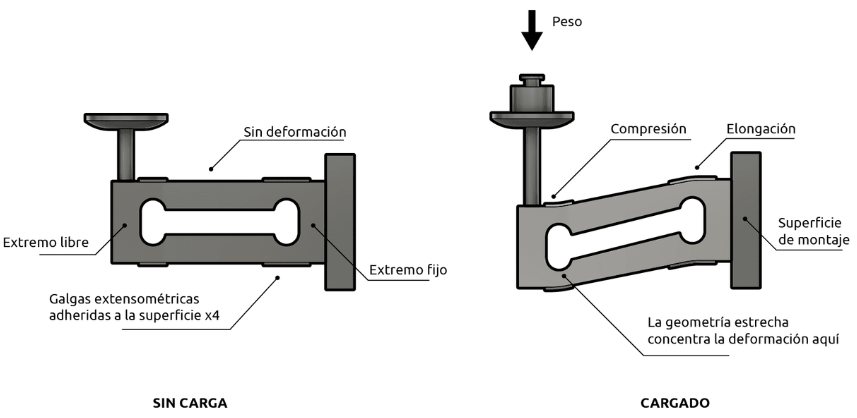
\includegraphics[width=\textwidth]{img/EA-celulaCarga.png}
		\caption[Funcionamiento de una célula de carga]{Funcionamiento de una célula de carga. Fuente: \parencite{muller_2010_load_cells}}
		\label{fig:celula-carga}
	\end{minipage}
\end{figure}

\paragraph{Resistencia y tacto del pedal.}
Medir la fuerza no basta, ya que el pedal debe oponer una resistencia que se parezca a la del coche real. Hay tres soluciones, de menor a mayor complejidad:
\begin{itemize}
	\item \textbf{Muelles y elastómeros}: el muelle da una resistencia lineal y el elastómero, una resistencia progresiva que se endurece al final del recorrido, como un circuito de freno real.
	Combinando muelles y elastómeros de distinta dureza se ajusta el tacto. Es la solución de la mayoría de las pedaleras con célula de carga.
	\item \textbf{Amortiguación hidráulica}: añade un amortiguador que reproduce la resistencia del líquido de frenos y suaviza la respuesta del pedal, como en las pedaleras de gama alta de Simagic o
	Heusinkveld.
	\item \textbf{Pedales activos}: un servomotor controlado por software genera la resistencia, lo que permite cambiar el tacto en cada coche y transmitir efectos como el ABS o el bloqueo de las ruedas. Es la tecnología de los pedales de Simucube y la más cara del mercado.
\end{itemize}

\paragraph{Retroalimentación háptica.}
Los pedales activos son la única solución que integra la resistencia y los efectos en el propio pedal, pero su precio los deja fuera del alcance de la mayoría. La alternativa es añadir a una pedalera pasiva
un actuador háptico que haga vibrar el pedal. El piloto no recibe la fuerza del coche, pero sí la información que más necesita en la frenada y la aceleración: la vibración en el freno indica que actúa
el ABS o que las ruedas se bloquean, y en el acelerador, que las ruedas traseras patinan. Se utilizan tres tipos de actuador \parencite{choi_2013_vibrotactile}:
\begin{itemize}
	\item \textbf{Motores de masa excéntrica (ERM)}: pequeños motores de corriente continua con una masa
	descentrada en el eje, como los de los mandos de consola. Son baratos y fáciles de controlar, pero tardan en arrancar y detenerse, y la frecuencia y la intensidad de la vibración están ligadas entre sí. Es la solución que incorporan, por ejemplo, el freno y el acelerador de las ClubSport Pedals~V3 de Fanatec \parencite{fanatec_web}.
	\item \textbf{Actuadores lineales}: un campo magnético desplaza una masa en línea recta, como en un altavoz. Responden más rápido y permiten controlar la frecuencia con independencia de la intensidad,
	lo que hace distinguible, por ejemplo, el ABS del paso por un piano. Es el principio del Haptic Pedal Reactor (P-HPR) de Simagic, que se monta detrás de la plataforma del pedal y alcanza hasta
	50~Hz \parencite{simagic_web}.
	\item \textbf{Transductores táctiles} (\textit{bass shakers}): actuadores de audio de baja frecuencia que se fijan al \textit{cockpit} o al asiento. Transmiten vibraciones a todo el puesto, como el motor o los baches, más que efectos concretos de un pedal.
\end{itemize}
Estos efectos no se calculan en la pedalera, sino a partir de la telemetría que publica el simulador. Programas como SimHub, mediante su módulo ShakeIt, leen esos datos y generan la señal de cada
actuador \parencite{simhub_web}. En las soluciones de fabricación propia, un microcontrolador recibe esa señal por USB y gobierna los motores mediante un controlador de potencia, lo que permite añadir vibración a una pedalera casera por muy poco coste.

\paragraph{Conexión y configuración.}
Sea cual sea el sensor, la pedalera se presenta al ordenador como un dispositivo USB HID con un eje por pedal, sin necesidad de controladores específicos. Sobre la lectura del sensor se aplican después ajustes por software: una calibración de los extremos, zonas muertas para evitar lecturas no deseadas en reposo y curvas de respuesta que modifican la relación entre la entrada del piloto y el valor enviado al simulador. Estos ajustes se realizan en el software de cada fabricante o, en las soluciones de fabricación propia, en el propio firmware del microcontrolador.
\subsection{Aros}
\label{sec:aros}

El aro es la parte del volante que el piloto sujeta y la única pieza del puesto que está en contacto permanente con sus manos. Cumple dos funciones: transmitir a las manos el par que genera la base y reunir los mandos que el piloto acciona sin soltar el volante. Por eso su diseño combina un componente mecánico, la forma, el tamaño y la rigidez del aro, con uno electrónico, los botones, levas y luces que lo convierten en un periférico de entrada.

\paragraph{Formatos.}
La forma del aro depende del tipo de coche que se quiere reproducir. Los aros redondos, de unos 300 a 350~mm de diámetro, corresponden a los turismos, los GT y los coches de rally, en los que el volante gira más de media vuelta y el piloto cambia la posición de las manos. Los aros de tipo Fórmula, más pequeños y con forma de mariposa, reproducen los de los monoplazas y los prototipos de resistencia: el giro es tan reducido que las manos no se mueven del aro, y casi todos los mandos del coche se concentran en él. Entre ambos se sitúan los aros de tipo GT con la parte superior abierta o plana, cada vez más habituales en los GT3 actuales, que combinan un giro amplio con una botonera completa, como el Podium Steering Wheel BMW~M4~GT3 de Fanatec \parencite{fanatec_web}.

\paragraph{Mandos.}
Un aro de competición reproduce los controles que el piloto usa durante la carrera. Los más sencillos son los pulsadores, que se asignan a funciones como el limitador de velocidad en el \textit{pit lane}, la radio o el cambio de página de la pantalla. Los selectores rotativos permiten ajustar parámetros por pasos, como el reparto de frenada, el control de tracción o el ABS, y los \textit{encoders} incrementales, que giran sin tope y envían un pulso por cada paso, se usan para recorrer menús o ajustar valores de forma continua. Detrás del aro se montan las levas de cambio y, en los aros de tipo Fórmula, dos levas analógicas de embrague que el piloto usa en las salidas para dosificar la tracción. Para detectar la posición de las levas se emplean microinterruptores, que dan un clic mecánico definido, o sensores Hall y magnéticos, que no se desgastan y permiten una lectura analógica \parencite{ramsden_2006_hall}.

\paragraph{Información al piloto.}
Además de recoger órdenes, el aro informa al piloto. La mayoría de los aros de gama media y alta incorpora una fila de LEDs que se encienden progresivamente con las revoluciones del motor e indican el momento del cambio de marcha, o dan información como las banderas en pista o el estado de la batería, según los gustos de cada piloto; los de gama alta añaden una pantalla con la marcha, los tiempos por vuelta o el estado de los neumáticos. Igual que la vibración de los pedales (sección~\ref{sec:pedaleras}), estos datos no los genera el aro, sino que proceden de la telemetría del simulador, leída por el software del fabricante o por programas como SimHub.

\paragraph{Electrónica.}
Un aro reúne fácilmente más de veinte entradas, demasiadas para conectar cada una a un pin del microcontrolador. La solución habitual es organizar los pulsadores en una matriz de filas y columnas, en la que el microcontrolador activa las filas una a una y lee las columnas para saber qué pulsador está pulsado. Con una matriz de 5$\times$5 se leen 25 pulsadores con solo 10 pines, y añadiendo un diodo en serie con cada pulsador se evitan las lecturas falsas cuando se pulsan varios a la vez. Los \textit{encoders} y las levas analógicas se leen aparte, y el microcontrolador presenta todo el conjunto al ordenador como un único dispositivo USB HID con botones y ejes, como permite la biblioteca Arduino Joystick sobre placas ATmega32U4 (sección~\ref{sec:soluciones-abiertas}).

\paragraph{Conexión con la base.}
El aro se une a la base mediante un anclaje rápido que transmite el par y, en los ecosistemas comerciales, también la alimentación y los datos a través de contactos eléctricos propios de cada marca. Como se vio en la sección~\ref{sec:productos-relacionados}, este es uno de los puntos en los que los fabricantes cierran su ecosistema: un aro de una marca solo funciona por completo sobre una base de la misma marca. La alternativa es separar ambas funciones: un anclaje puramente mecánico, compatible con el patrón de seis tornillos sobre un círculo de 70~mm habitual en los volantes de competición, y una conexión independiente del aro al ordenador por USB o por radio, como hacen Simucube y la mayoría de los aros de fabricación propia \parencite{simracingcockpit_qr, simucube_web}.

\paragraph{Materiales y fabricación.}
El aro debe ser rígido, porque cualquier flexión resta precisión a la información que llega de la base, y ligero, porque su inercia se suma a la que tiene que mover el motor. Los aros comerciales combinan una placa frontal de aluminio o fibra de carbono con empuñaduras de piel, ante o goma. En los aros de fabricación propia, la impresión 3D permite reproducir la forma y la disposición de mandos de un volante real a bajo coste, reservando las piezas metálicas para las zonas que soportan el par.

\subsection{Software de apoyo para el piloto}
\label{sec:software-apoyo}

Además del simulador y del software de configuración de cada fabricante, el piloto utiliza un conjunto de programas que le ayudan durante la carrera y después de ella. Ninguno modifica la física del simulador: todos trabajan sobre los datos que este publica, y cumplen funciones que en un equipo real reparten el ingeniero de pista, el \textit{spotter} y el analista de datos.

\paragraph{La telemetría como punto de partida.}
Todos estos programas dependen de la telemetría, el conjunto de datos que el simulador calcula en cada instante: velocidad, revoluciones, marcha, posición de los pedales y del volante, temperaturas y presiones de los neumáticos, combustible, posición en carrera o diferencias con los rivales. Los simuladores la ponen a disposición de otros programas de dos formas: escribiéndola en una zona de memoria compartida que cualquier aplicación del mismo ordenador puede leer, como hacen iRacing, Assetto Corsa Competizione o rFactor~2, o enviándola en paquetes UDP por la red, como la saga de Fórmula~1 o Gran Turismo~7, lo que permite leerla también desde otro dispositivo \parencite{kunos_acc_shared_memory, ea_f1_25_udp, gtplanet_gt7_telemetry}. Cada simulador usa además su propio formato, por lo que las herramientas de apoyo necesitan un adaptador para cada título.

\paragraph{Información en tiempo real.}
El primer grupo de programas muestra al piloto la información que necesita mientras conduce. La herramienta más extendida es SimHub, gratuita con una licencia opcional de pago, que reúne en una sola aplicación las pantallas de datos (\textit{dashes}), que pueden mostrarse en una pantalla auxiliar, en una tableta o superpuestas al juego, el control de los LEDs de revoluciones y banderas de aros y pantallas, y el módulo ShakeIt, que genera las vibraciones de pedales y asientos descritas en la sección~\ref{sec:pedaleras} \parencite{simhub_web}. Además, permite conectar placas Arduino para construir indicadores propios, lo que la ha convertido en la base de buena parte del hardware de fabricación propia. Z1 Dashboard cubre una función parecida, centrada en las pantallas y los LEDs \parencite{z1_web}.

\paragraph{Ingeniero y \textit{spotter} por voz.}
En una carrera real, el piloto recibe por radio la información que no puede leer mientras conduce. Crew Chief reproduce ese papel en el simulador: es una aplicación gratuita que actúa como ingeniero y como \textit{spotter}, avisa de los coches que se encuentran a los lados, de las banderas, de las diferencias con los rivales o del combustible restante, y con reconocimiento de voz permite preguntarle por esos datos sin soltar el volante. Funciona con la mayoría de los simuladores de PC, como iRacing, Assetto Corsa Competizione o rFactor~2 \parencite{crewchief_web}.

\paragraph{Análisis de telemetría.}
Después de la sesión, el piloto compara sus vueltas para encontrar dónde pierde tiempo, igual que hacen los ingenieros con los datos del coche real. Para ello se usan las mismas herramientas que en la competición profesional: Assetto Corsa Competizione exporta su telemetría en el formato de MoTeC~i2, el programa de análisis de datos más extendido en el automovilismo, e iRacing ofrece gratis a sus usuarios Pi Toolbox, el software de análisis de Cosworth, que lee directamente sus archivos \parencite{acc_motec_blog, motec_i2, cosworth_iracing}. Junto a ellas han surgido plataformas pensadas para el simracing, como Garage~61, que permite comparar las vueltas propias con las de otros pilotos en el mismo coche, o Coach Dave Delta, que además instala reglajes y señala automáticamente en qué curvas se pierde tiempo \parencite{garage61_web, coachdave_delta}.

\paragraph{Limitaciones.}
Estas herramientas cubren entre todas las necesidades del piloto, pero lo hacen por separado. Cada una tiene su propia instalación, su configuración y sus perfiles, y en un mismo puesto conviven a menudo SimHub, Crew Chief, un programa de análisis y el software de cada fabricante de periféricos. Ninguna conoce el hardware sobre el que se ejecuta: SimHub puede encender los LEDs de un aro, pero no ajusta el force feedback de la base ni la curva del freno, que siguen dependiendo de la aplicación de cada marca. Esta fragmentación es la que intenta resolver el configurador de este trabajo, que reúne en una sola aplicación las pantallas, las luces, el ingeniero por voz, la estrategia y el análisis de telemetría, y que conoce los periféricos a los que se conecta (sección~\ref{sec:estado-arte-conclusion}).
\section{Productos relacionados}
\label{sec:productos-relacionados}

El mercado de periféricos de simracing reúne hoy a un número creciente de fabricantes, con gamas que van desde equipos de entrada orientados al jugador ocasional hasta material profesional usado por pilotos y equipos de competición. Junto a esta oferta comercial ha crecido una comunidad de proyectos de código abierto y de fabricación propia (\textit{Do It Yourself}, DIY) que permite a un usuario construir sus propios periféricos a partir de controladoras de motor genéricas, microcontroladores y piezas impresas en 3D.

Esta sección analiza ambos enfoques. La sección~\ref{sec:mercado-perifericos} cuantifica el mercado y lo divide por gamas, la sección~\ref{sec:soluciones-comerciales} recoge las principales marcas comerciales (Fanatec, Simucube, Moza, Simagic y Heusinkveld) y la sección~\ref{sec:soluciones-abiertas}, las alternativas abiertas más extendidas (ODrive, OpenFFBoard, FFBeast y la biblioteca Arduino Joystick). Para que la comparación sea homogénea, cada solución se evalúa con los mismos criterios, derivados de los fundamentos técnicos de la sección~\ref{sec:fundamentos-tecnicos}:
\begin{itemize}
	\item \textbf{Transmisión y par}: tipo de transmisión de la base y par máximo disponible.
	\item \textbf{Medida en los pedales}: freno por recorrido o por fuerza, y tipo de sensor.
	\item \textbf{Apertura}: si el firmware y el diseño son abiertos o propietarios.
	\item \textbf{Ecosistema}: software de configuración, conexión entre aro y base, y compatibilidad con otras marcas.
	\item \textbf{Alcance}: qué periféricos cubre (base, aro, pedalera) y qué software de apoyo al piloto incluye.
	\item \textbf{Coste} aproximado.
\end{itemize}
El resultado se resume en la tabla~\ref{tab:comparativa}, que sirve de base para la conclusión del capítulo.

\subsection{Mercado de periféricos}
\label{sec:mercado-perifericos}

Cuantificar el mercado del simracing no es sencillo, porque los informes sectoriales no comparten una definición común. Los que se limitan a los simuladores de carreras, es decir, al hardware y al software de simulación, lo estiman en torno a 0,9~miles de millones de dólares en 2025, con un crecimiento anual del orden del 7--8\,\% \parencite{tbrc_2026_racing_sim}. Los que incluyen también los videojuegos de carreras en general elevan la cifra hasta unos 3,8~miles de millones de dólares en el mismo año, con previsiones que la sitúan cerca de los 7,7~miles de millones en 2035 \parencite{mri_2025_car_racing_games}. La diferencia entre ambas estimaciones confirma la distinción entre juegos y simuladores de la sección~\ref{sec:simracing-mercado}: el simracing, entendido como simulación con periféricos específicos, es una fracción del mercado de los juegos de carreras, pero una fracción con un gasto por usuario mucho mayor.

La figura~\ref{fig:mercado-estimaciones} compara las estimaciones de tres consultoras para el mercado de simuladores de carreras: aunque difieren en el punto de partida y en el horizonte, todas prevén que el mercado al menos se duplique en la próxima década.

% Estimaciones del mercado de simuladores de carreras según cada consultora (miles de millones de dólares).
% Datos y fuentes (valor de partida -> previsión):
%   MarketsandMarkets         0,50 (2024) -> 1,10 (2030)
%   Mordor Intelligence       0,98 (2025) -> 2,04 (2030)
%   Market Research Future    1,05 (2025) -> 4,31 (2035)
\begin{figure}[htbp]
	\centering
	\begin{tikzpicture}
		\begin{axis}[
			grafica,
			scale only axis, width=0.5\linewidth, height=5.5cm,
			xbar=3pt, bar width=8pt,
			xmin=0, xmax=5.2,
			area legend,
			legend style={/tikz/every even column/.append style={column sep=10pt}},
			xmajorgrids, ymajorgrids=false,
			axis lines*=left,
			symbolic y coords={Market Research Future,Mordor Intelligence,MarketsandMarkets},
			ytick=data,
			y dir=reverse,
			enlarge y limits=0.15,
			xlabel={Tamaño del mercado (miles de millones de dólares)},
			point meta=explicit symbolic,
			nodes near coords,
			every node near coord/.append style={font=\scriptsize, text=black, anchor=west},
			legend style={at={(0.5,1.02)}, anchor=south},
		]
			\addplot[fill=serie1, draw=none] coordinates {
				(0.50,MarketsandMarkets) [0,50 (2024)]
				(0.98,Mordor Intelligence) [0,98 (2025)]
				(1.05,Market Research Future) [1,05 (2025)]
			};
			\addplot[fill=serie2, draw=none] coordinates {
				(1.10,MarketsandMarkets) [1,10 (2030)]
				(2.04,Mordor Intelligence) [2,04 (2030)]
				(4.31,Market Research Future) [4,31 (2035)]
			};
			\legend{Valor de partida, Previsión}
		\end{axis}
	\end{tikzpicture}
	\caption[Estimaciones del mercado de simuladores de carreras]{Estimaciones del tamaño del mercado de simuladores de carreras según tres consultoras, con el año de cada valor. Fuente: resúmenes públicos de los informes de MarketsandMarkets, Mordor Intelligence y Market Research Future \parencite{marketsandmarkets_racing_sim, mordor_2025_racing_sim, mrfr_2025_racing_sim}.}
	\label{fig:mercado-estimaciones}
\end{figure}


Coinciden, en cambio, en los factores que explican el crecimiento: la popularidad de los eSports, la implicación de pilotos y equipos profesionales y la mejora del hardware disponible para el consumidor \parencite{mordor_2025_racing_sim}. Este último factor es el más relevante para este trabajo. La llegada de las bases \textit{direct drive} y de las pedaleras con célula de carga a precios de consumo (sección~\ref{sec:soluciones-comerciales}) ha hecho que el periférico sea el componente que más pesa en el coste de un ecosistema propio: un aficionado puede pagar una suscripción mensual o simuladores por decenas de euros, pero un ecosistema completamente equipado con base, aro y pedalera de gama media supera con facilidad los mil euros.

La evolución de Fanatec, el mayor fabricante del sector, ilustra este auge del hardware (figura~\ref{fig:fanatec-facturacion}): su facturación se multiplicó por más de diez entre 2016 y 2022, con un salto del 132\,\% en 2020.

% Facturación anual de Endor AG, empresa propietaria de Fanatec (millones de euros).
% Datos y fuentes:
%   2016-2021  Börsengeflüster, "Endor: Voll auf Wachstumskurs" (tabla de Umsatzerlöse)
%   2020       Endor AG, cifras preliminares 2020: 90 M€ frente a 38,8 M€ en 2019 (+132 %)
%   2021       Endor AG, cifras preliminares 2021: un 10 % menos por falta de suministro
%   2022       TraderFox (119,19 M€); Landshuter Rundschau cita 119 M€
\begin{figure}[htbp]
	\centering
	\begin{tikzpicture}
		\begin{axis}[
			grafica,
			ybar, bar width=18pt,
			ymin=0, ymax=135,
			xtick=data,
			xticklabel style={/pgf/number format/1000 sep={}},
			ylabel={Facturación (millones de euros)},
			nodes near coords,
			every node near coord/.append style={font=\footnotesize, text=black,
				/pgf/number format/fixed, /pgf/number format/precision=1},
			enlarge x limits=0.08,
		]
			\addplot[fill=serie1, draw=none]
				coordinates {
					(2016, 10.2) (2017, 18.4) (2018, 22.1) (2019, 38.8)
					(2020, 90.2) (2021, 81.3) (2022, 119.2)
				};
		\end{axis}
	\end{tikzpicture}
	\caption[Facturación anual de Endor AG (Fanatec)]{Facturación anual de Endor AG, la empresa propietaria de Fanatec, entre 2016 y 2022. El salto de 2020 coincide con la pandemia y la caída de 2021 se debe a la falta de suministro de componentes. Fuente: comunicados de resultados de Endor AG \parencite{endor_web}.}
	\label{fig:fanatec-facturacion}
\end{figure}


\paragraph{Segmentación del mercado de periféricos.}
De lo anterior se desprende una segmentación por niveles que se mantiene en el resto de la sección:
\begin{itemize}
	\item \textbf{Gama de entrada}: volantes con transmisión por engranajes o correa y pedales que miden el recorrido, pensados para el jugador ocasional y compatibles con consolas.
	\item \textbf{Gama media}: bases \textit{direct drive} de bajo y medio par y pedaleras con célula de carga, donde se concentra hoy el crecimiento del sector.
	\item \textbf{Gama alta y profesional}: bases de alto par, pedales hidráulicos o activos, réplicas de volantes reales y simuladores completos con plataformas de movimiento, usados por equipos, academias y pilotos profesionales.
\end{itemize}
El salto entre la gama de entrada y la media es el más significativo tanto en experiencia como en precio, y es el espacio en el que se sitúa la propuesta de este trabajo.

\subsection{Productos comerciales}
\label{sec:soluciones-comerciales}

La oferta comercial se concentra en pocos fabricantes, que en los últimos años han llevado el \textit{direct drive} de la gama profesional a la de entrada. Los cinco que se analizan cubren todo el espectro de precios y los dos modelos de negocio dominantes: el ecosistema completo, en el que una misma marca vende base, aros y pedaleras, y el fabricante especializado en un solo tipo de periférico.

\paragraph{Fanatec.}
Fanatec, la marca de simracing de la alemana Endor~AG, ha sido durante años el fabricante de mayor volumen del sector, con unas ventas cercanas a los 110 millones de dólares en 2023. En 2024, dentro del procedimiento de insolvencia de Endor, la compró Corsair, y hoy forma parte de un grupo de periféricos para videojuegos \parencite{businesswire_2024_corsair_fanatec}.

\textit{Colaboraciones con marcas reales.} Fanatec ha construido su imagen sobre licencias del mundo del motor: colabora con Porsche desde 2006 y con BMW desde 2011. El caso más relevante es el Podium Steering Wheel BMW~M4~GT3 (2022), que no es una réplica: Fanatec y BMW M Motorsport lo desarrollaron, con pilotos oficiales como Philipp Eng, para el propio coche de competición, y la versión de simulación es el mismo volante, con los mismos mandos y el mismo tacto que el piloto encuentra en pista \parencite{fanatec_web}. Desde 2018 es además socio de las F1 Esports Series, lo que le permite vender aros con licencia de la Fórmula~1 \parencite{fanatec_web}.

\textit{Bases.} Todo el catálogo es \textit{direct drive} y comparte el anclaje rápido QR2. La gama se escalona por par, desde la CSL~DD (5~N\,m, ampliable a 8~N\,m) hasta la Podium~DD (25~N\,m sostenidos y picos de 33~N\,m), que en 2026 sustituyó a la Podium~DD2 \parencite{fanatec_web}. Tras la bajada de precios de principios de 2026, la gama va de unos 330 a 1\,100~euros (tabla~\ref{tab:fanatec}).

\begin{table}[htbp]
	\centering
	\caption[Bases \textit{direct drive} de Fanatec (precios oficiales en euros, 2026)]{Bases \textit{direct drive} de Fanatec (precios oficiales en euros, 2026). Fuente: \parencite{fanatec_web}}
	\label{tab:fanatec}
	\begin{tabular}{|l|c|c|l|}
		\hline
		\textbf{Base} & \textbf{Par (N\,m)} & \textbf{Precio (\euro)} & \textbf{Plataformas} \\
		\hline
		CSL DD        & 5 (8 con kit) & 329,95    & PC, Xbox \\
		GT DD Pro     & 8             & 499,95    & PC, PlayStation \\
		ClubSport DD  & 12            & 599,95    & PC \\
		ClubSport DD+ & 15            & 799,95    & PC, PlayStation \\
		Podium DD     & 25 (33 pico)  & 1\,099,95 & PC, Xbox \\
		\hline
	\end{tabular}
\end{table}

\textit{Pedaleras.} Las CSL Pedals de entrada miden el freno por recorrido, aunque con sensores Hall sin contacto en lugar de potenciómetros, y admiten un kit de célula de carga. La célula viene de serie en las gamas superiores: las ClubSport Pedals~V3 miden hasta 90~kg y las Podium Pedals, de 2026, hasta 150~kg en el pedal \parencite{fanatec_web}. Como en las bases, el sensor y la fuerza máxima marcan la diferencia entre gamas (tabla~\ref{tab:fanatec-pedales}).

\begin{table}[htbp]
	\centering
	\caption[Pedaleras de Fanatec (precios oficiales en euros, 2026)]{Pedaleras de Fanatec (precios oficiales en euros, 2026). Fuente: \parencite{fanatec_web}}
	\label{tab:fanatec-pedales}
	\small
	\begin{tabular}{|l|l|c|c|}
		\hline
		\textbf{Pedalera} & \textbf{Sensor del freno} & \textbf{Fuerza máx. (kg)} & \textbf{Precio (\euro)} \\
		\hline
		CSL Pedals                        & Hall (por recorrido) & --  & 99,95 \\
		CSL Pedals LC                     & Célula de carga      & --  & 179,90 \\
		CSL Elite Pedals V2               & Célula de carga      & --  & 299,95 \\
		ClubSport Pedals V3               & Célula de carga      & 90  & 329,95 \\
		ClubSport Pedals V3 Inverted      & Célula de carga      & 90  & 429,99 \\
		Podium Pedals Sport (2 pedales)   & Célula de carga      & 150 & 599,95 \\
		Podium Pedals Formula (2 pedales) & Célula de carga      & 150 & 699,95 \\
		\hline
	\end{tabular}
\end{table}

\textit{Aros y ecosistema.} Los aros muestran el peso de las licencias en el precio (tabla~\ref{tab:fanatec-aros}): los de estilo GT o Fórmula cuestan entre 200 y 360~euros, mientras que el BMW~M4~GT3, que procede del coche real, ronda los 1\,500, más que la base más potente de la marca. Todos se conectan por el QR2, que lleva la alimentación y los datos del aro, y se configuran desde la aplicación de Fanatec. Es el ecosistema más completo del mercado y también el más cerrado, y su principal ventaja es la compatibilidad oficial con consolas, poco habitual en el resto de marcas.

\begin{table}[htbp]
	\centering
	\caption[Selección de aros de Fanatec (precios oficiales en euros, 2026)]{Selección de aros de Fanatec (precios oficiales en euros, 2026). Fuente: \parencite{fanatec_web}}
	\label{tab:fanatec-aros}
	\small
	\begin{tabular}{|l|l|l|c|}
		\hline
		\textbf{Aro} & \textbf{Estilo} & \textbf{Licencia} & \textbf{Precio (\euro)} \\
		\hline
		CSL Steering Wheel GT3                     & GT      & --        & 199,95 \\
		ClubSport Steering Wheel F1 Esports V2     & Fórmula & Formula 1 & 239,95 \\
		CSL Elite Steering Wheel Porsche Vision GT & GT      & Porsche   & 349,95 \\
		ClubSport Steering Wheel Formula V2.5      & Fórmula & --        & 359,95 \\
		Podium Steering Wheel BMW M4 GT3           & GT      & BMW M Motorsport\textsuperscript{*} & 1\,499,95 \\
		\hline
		\multicolumn{4}{l}{\footnotesize \textsuperscript{*} Volante desarrollado para el coche de competición real.} \\
	\end{tabular}
\end{table}



\paragraph{Simucube.}
Simucube nace de Granite Devices, una empresa finlandesa de servoaccionamientos industriales. En 2016 lanzó por micromecenazgo el SimuCUBE~1, una controladora de force feedback surgida de la comunidad de simracing de fabricación propia, y con la Simucube~2, en 2019, pasó a dedicarse por completo a la simulación \parencite{simucube_web}. Es el único fabricante analizado que procede del control industrial de motores, y su prestigio se apoya en la calidad de ese control.

\textit{Colaboraciones con equipos reales.} En lugar de licencias de fabricantes, Simucube se apoya en alianzas con equipos: es socio oficial de Verstappen Sim Racing, cuyos pilotos usan solo su material, y mantiene un acuerdo técnico con Rodin Motorsport, que emplea sus productos en su simulador \textit{driver-in-the-loop} y en la preparación de sus pilotos \parencite{simucube_web}.

\textit{Bases.} La Simucube~2, durante años la referencia de la gama alta, ha dado paso a la Simucube~3, cuyos pedidos se abrieron en octubre de 2025. Estrena motor y se ofrece en Sport (15~N\,m), Pro (25~N\,m) y Ultimate (35~N\,m), el par más alto de los fabricantes analizados \parencite{simucube_web}. También es la más cara: la Pro cuesta unos 1\,490~euros, frente a los 1\,100 de la Podium~DD de Fanatec con el mismo par, y la Ultimate supera los 3\,200 (tabla~\ref{tab:simucube}).

\begin{table}[htbp]
	\centering
	\caption[Bases \textit{direct drive} de Simucube (precios oficiales en euros, 2026)]{Bases \textit{direct drive} de Simucube (precios oficiales en euros, 2026). Fuente: \parencite{simucube_web}}
	\label{tab:simucube}
	\small
	\begin{tabular}{|l|c|c|l|}
		\hline
		\textbf{Base} & \textbf{Par (N\,m)} & \textbf{Precio (\euro)} & \textbf{Estado} \\
		\hline
		Simucube 3 Sport    & 15 & 1\,246,80 & Actual \\
		Simucube 3 Pro      & 25 & 1\,486,80 & Actual \\
		Simucube 3 Ultimate & 35 & 3\,214,80 & Actual \\
		Simucube 2 Sport    & 17 & --        & Retirada \\
		Simucube 2 Pro      & 25 & --        & Retirada \\
		Simucube 2 Ultimate & 32 & --        & Retirada \\
		\hline
	\end{tabular}
\end{table}

\textit{Pedaleras.} En lugar de pedaleras convencionales fabrica pedales activos: en el ActivePedal la resistencia la genera un servomotor controlado por software, lo que permite cambiar la dureza y la curva en cada coche y transmitir efectos como el ABS o el bloqueo de la rueda. Es el principio del force feedback aplicado al pedal. Cada pedal cuesta entre unos 1\,090 y 2\,500~euros según la versión \parencite{simucube_web}, más que muchas bases \textit{direct drive} completas (tabla~\ref{tab:simucube-otros}).

\textit{Aros y ecosistema.} Sus aros, como el Tahko~GT-21 o el Savu Pro, son inalámbricos: el anclaje rápido es solo mecánico y el aro se comunica con la base por radio, lo que también facilita montar aros de terceros conectados por USB. Todo se configura con Simucube Tuner, y la marca no ofrece compatibilidad con consolas.

\begin{table}[htbp]
	\centering
	\caption[Pedales y aros de Simucube (precios en euros, 2026)]{Pedales y aros de Simucube (precios en euros, 2026). Fuente: \parencite{simucube_web}}
	\label{tab:simucube-otros}
	\small
	\begin{tabular}{|l|l|c|}
		\hline
		\textbf{Producto} & \textbf{Tipo} & \textbf{Precio (\euro)} \\
		\hline
		ActivePedal Sport        & Pedal activo (servomotor) & 1\,089,99 \\
		ActivePedal Pro          & Pedal activo (servomotor) & $\approx$\,1\,760 \\
		ActivePedal Ultimate     & Pedal activo (servomotor) & $\approx$\,2\,500 \\
		Tahko GT-21              & Aro GT inalámbrico        & 829,99 \\
		Savu Pro                 & Aro Fórmula inalámbrico   & desde 1\,259,99 \\
		\hline
		\multicolumn{3}{l}{\footnotesize Precio de los pedales por unidad.} \\
	\end{tabular}
\end{table}

\paragraph{Moza.}
Moza Racing es la división de simracing de Gudsen Technology, una empresa de Shenzhen fundada en 2012 y conocida por sus estabilizadores de cámara (\textit{gimbals}). En 2021 llevó su experiencia en control de motores a la simulación con un ecosistema \textit{direct drive} completo \parencite{moza_web}, y en cinco años se ha convertido en el principal competidor de Fanatec gracias a sus precios.

\textit{Colaboraciones con marcas reales.} Como Fanatec, apuesta por las licencias: vende aros oficiales de Lamborghini y de Porsche, cuyo Mission~R se reprodujo a partir de los datos CAD del fabricante, y en la Gamescom de 2026 presentó otros de Porsche, Mercedes-Benz y Ford. Desde agosto de 2026 es además socio oficial de la Gran Turismo World Series \parencite{moza_web}.

\textit{Bases.} Tiene la escalera de par más fina del mercado, con una base cada 3 o 4~N\,m desde la R3 (3,9~N\,m) hasta la R25 Ultra, y los precios más bajos de los fabricantes analizados: la R16 Ultra cuesta unos 550~euros, menos que la ClubSport~DD de Fanatec de 12~N\,m \parencite{moza_web} (tabla~\ref{tab:moza}).

\begin{table}[htbp]
	\centering
	\caption[Bases \textit{direct drive} de Moza (precios oficiales, 2026)]{Bases \textit{direct drive} de Moza (precios oficiales, 2026). Fuente: \parencite{moza_web}}
	\label{tab:moza}
	\small
	\begin{tabular}{|l|c|c|}
		\hline
		\textbf{Base} & \textbf{Par (N\,m)} & \textbf{Precio} \\
		\hline
		R3 (pack con aro y pedales)  & 3,9 & 399~\$ \\
		R5 Pro (pack)                & 6   & 419~\euro \\
		R9 V3                        & 9   & 399~\euro \\
		R12 V2                       & 12  & 529~\euro \\
		R16 Ultra                    & 16  & 549~\euro \\
		R21 Ultra                    & 21  & 699~\$ \\
		R25 Ultra                    & --  & 899~\$ \\
		\hline
		\multicolumn{3}{l}{\footnotesize En dólares cuando no hay precio oficial en euros.} \\
	\end{tabular}
\end{table}

\textit{Pedaleras.} La SR-P de entrada usa un sensor de fuerza de 100~kg en el freno, y la CRP2 de gama alta una célula de carga de 200~kg, comparable a la de las Podium Pedals de Fanatec, que cuestan unos 250~euros más \parencite{moza_web} (tabla~\ref{tab:moza-pedales-aros}).

\textit{Aros y ecosistema.} Combina aros propios, de unos 280 a 830~euros, con los licenciados, que llegan a los 1\,299~dólares del Porsche Mission~R. Como en Fanatec, el anclaje rápido lleva la conexión eléctrica del aro, así que los aros Moza solo funcionan completos sobre bases Moza, y todo se configura desde su aplicación Pit House.

\begin{table}[htbp]
	\centering
	\caption[Pedaleras y aros de Moza (precios oficiales, 2026)]{Pedaleras y aros de Moza (precios oficiales, 2026). Fuente: \parencite{moza_web}}
	\label{tab:moza-pedales-aros}
	\small
	\begin{tabular}{|l|l|l|c|}
		\hline
		\textbf{Producto} & \textbf{Tipo} & \textbf{Licencia / sensor} & \textbf{Precio} \\
		\hline
		SR-P               & Pedalera     & Sensor de 100 kg        & 159~\euro \\
		CRP2               & Pedalera     & Célula de carga 200 kg  & 449~\euro \\
		KS                 & Aro GT       & --                      & 279~\euro \\
		GS V2P             & Aro GT       & --                      & 439~\euro \\
		FSR2               & Aro Fórmula  & --                      & 699~\euro \\
		Vision GS          & Aro GT       & --                      & 829~\euro \\
		Lamborghini Revuelto & Aro GT     & Lamborghini             & 399~\$ \\
		Porsche Mission R  & Aro GT       & Porsche                 & 1\,299~\$ \\
		\hline
	\end{tabular}
\end{table}

\paragraph{Simagic.}
Simagic es un fabricante chino de gama media-alta, con buena relación calidad-precio, que hasta 2026 prefirió asociarse con competiciones y pilotos antes que con fabricantes de automóviles.

\textit{Colaboraciones con marcas reales.} Desde 2023 es proveedor oficial de la Formula DRIFT, el campeonato estadounidense de drift, con cuyos pilotos ha calibrado su force feedback, y en 2026 renovó el acuerdo por varios años. En octubre de 2026 anunció su primer volante licenciado, el del Aston Martin Valkyrie, al que seguirá el del KTM X-Bow~GT2 \parencite{simagic_web}.

\textit{Bases.} La familia Alpha EVO va de la Sport (9~N\,m) a la Ultra (28~N\,m), por entre unos 400 y 970~euros \parencite{simagic_web}. Por par y precio se sitúa entre Moza y Fanatec: la Ultra ofrece más par que la Podium~DD por unos 130~euros menos (tabla~\ref{tab:simagic}).

\begin{table}[htbp]
	\centering
	\caption[Bases \textit{direct drive} de Simagic (precios en euros de distribuidor europeo, 2026)]{Bases \textit{direct drive} de Simagic (precios en euros de distribuidor europeo, 2026). Fuente: \parencite{simagic_web}}
	\label{tab:simagic}
	\small
	\begin{tabular}{|l|c|c|}
		\hline
		\textbf{Base} & \textbf{Par (N\,m)} & \textbf{Precio (\euro)} \\
		\hline
		Alpha EVO Sport & 9  & 396,69 \\
		Alpha EVO       & 12 & 553,71 \\
		Alpha EVO Pro   & 18 & 702,47 \\
		Alpha EVO Ultra & 28 & 966,93 \\
		\hline
	\end{tabular}
\end{table}

\textit{Pedaleras.} La P1000 es modular, con una célula de carga de 100~kg en el freno que puede cambiarse por un sensor Hall, y la P2000 añade un sistema hidráulico que reproduce el tacto de un circuito de freno real, con células de 100 o 200~kg \parencite{simagic_web}. Es la única marca que lleva el freno hidráulico a la gama media (tabla~\ref{tab:simagic-pedales-aros}).

\textit{Aros y ecosistema.} Sus aros propios van de unos 300 a más de 500~euros, y el Aston Martin Valkyrie cuesta 799~dólares. Como el resto, usa un anclaje y un protocolo propios y se configura con su aplicación SimPro Manager.

\begin{table}[htbp]
	\centering
	\caption[Pedaleras y aros de Simagic (precios de 2026)]{Pedaleras y aros de Simagic (precios de 2026). Fuente: \parencite{simagic_web}}
	\label{tab:simagic-pedales-aros}
	\small
	\begin{tabular}{|l|l|l|c|}
		\hline
		\textbf{Producto} & \textbf{Tipo} & \textbf{Licencia / sensor} & \textbf{Precio} \\
		\hline
		P1000 (3 pedales)        & Pedalera     & Célula de carga 100 kg       & 469~\$ \\
		P2000 (3 pedales)        & Pedalera     & Hidráulica, célula de 200 kg & 689~\$ \\
		GT Neo                   & Aro GT       & --                           & $\approx$\,300~\euro \\
		FX Pro V2                & Aro Fórmula  & --                           & 549~\euro\textsuperscript{*} \\
		Aston Martin Valkyrie    & Aro GT       & Aston Martin                 & 799~\$ \\
		\hline
		\multicolumn{4}{l}{\footnotesize \textsuperscript{*} Sin IVA.} \\
	\end{tabular}
\end{table}

\paragraph{Heusinkveld.}
Heusinkveld representa el modelo especializado: solo fabrica pedaleras, palancas de cambio y frenos de mano. Svend y Niels Heusinkveld construyeron su primera pedalera en 2005 y, según la marca, fue la primera que medía el freno con una célula de carga \parencite{heusinkveld_web}, la idea que hoy es el estándar del sector.

\textit{Pedaleras.} Sus pedales reproducen la progresión de un freno real con elastómeros intercambiables de distinta dureza. La Sprint, su modelo más vendido, admite hasta 65~kg de fuerza en el pedal, y la Ultimate+ añade amortiguación hidráulica y llega a 140~kg, del orden de lo que exige el freno de un GT o de un Fórmula~1 real \parencite{heusinkveld_web}. La rigidez, el recorrido y la curva de respuesta se ajustan con su software SmartControl.

\textit{Precio y papel en el sector.} Sus precios son comparables a los de las pedaleras de gama alta de los ecosistemas completos (tabla~\ref{tab:heusinkveld}), pero no atan al usuario a una marca de base, porque la pedalera se conecta por USB de forma independiente. Su diseño ha servido de modelo, a escala reducida, para la pedalera de este trabajo.

\begin{table}[htbp]
	\centering
	\caption[Pedaleras de Heusinkveld (precios en euros, 2026)]{Pedaleras de Heusinkveld (precios en euros, 2026). Fuente: \parencite{heusinkveld_web}}
	\label{tab:heusinkveld}
	\small
	\begin{tabular}{|l|c|c|c|}
		\hline
		\textbf{Pedalera} & \textbf{Fuerza máx. (kg)} & \textbf{Amortiguación hidráulica} & \textbf{Precio (\euro)} \\
		\hline
		Sprint (2 pedales)     & 65  & No & 449\textsuperscript{*} \\
		Ultimate+ (2 pedales)  & 140 & Sí & desde 890 \\
		\hline
		\multicolumn{4}{l}{\footnotesize \textsuperscript{*} Sin IVA, tienda oficial.} \\
	\end{tabular}
\end{table}

\paragraph{Rasgos comunes.}
La tabla~\ref{tab:comerciales} resume las características de los cinco fabricantes. Todos han adoptado el \textit{direct drive} y la célula de carga como estándar de la gama media y alta, lo que confirma que son las tecnologías que determinan la calidad percibida. La comparación de precios muestra además dos estrategias: Moza y Simagic compiten en precio por N\,m, mientras que Fanatec y Simucube se apoyan en las licencias o en la calidad del control para justificar precios más altos. Al mismo tiempo, todos mantienen un firmware cerrado y un software de configuración propio, y los que venden ecosistemas completos condicionan la compatibilidad mediante el anclaje rápido y el protocolo de comunicación entre aro y base.

\begin{table}[htbp]
	\centering
	\caption[Comparativa de fabricantes comerciales de periféricos de simracing]{Comparativa de fabricantes comerciales de periféricos de simracing. Adaptado de: \parencite{fanatec_web, simucube_web, moza_web, simagic_web, heusinkveld_web}}
	\label{tab:comerciales}
	\small
	\begin{tabular}{|l|c|l|l|l|}
		\hline
		\textbf{Marca} & \textbf{Par (N\,m)} & \textbf{Pedales} & \textbf{Anclaje del aro} & \textbf{Software} \\
		\hline
		Fanatec     & 5--25   & Célula de carga      & Con contactos & Fanatec App \\
		Simucube    & 15--35  & Activos (servomotor) & Mecánico      & Simucube Tuner \\
		Moza        & 3,9--21 & Célula de carga      & Con contactos & Pit House \\
		Simagic     & 9--28   & Célula e hidráulica  & Propietario   & SimPro Manager \\
		Heusinkveld & --      & Célula de carga      & --            & SmartControl \\
		\hline
	\end{tabular}
\end{table}


\subsection{Proyectos open source y DIY}
\label{sec:soluciones-abiertas}

Frente a los ecosistemas cerrados de los fabricantes, la comunidad de simracing ha desarrollado proyectos para construir periféricos propios con componentes de propósito general. No son productos terminados, sino piezas: cada uno resuelve una parte del problema y deja al usuario la integración del resto. Para entender qué aporta cada uno conviene separar las tres capas que hay entre el simulador y el motor de una base, ya descritas en la sección~\ref{sec:bases-ffb} y representadas en la figura~\ref{fig:capas-abiertas}:
\begin{enumerate}
	\item \textbf{Comunicación con el ordenador}: presentarse por USB como dispositivo HID, enviar la posición del volante y recibir los efectos HID PID del simulador.
	\item \textbf{Cálculo del force feedback}: convertir esos efectos (fuerza constante, muelle, amortiguador, efectos periódicos) y los ajustes del usuario en una consigna de par, a una frecuencia muy superior a la del simulador.
	\item \textbf{Control del motor}: convertir la consigna de par en corrientes de fase mediante el control vectorial (FOC), leyendo la posición del rotor con el encoder.
\end{enumerate}
Los periféricos sin motor, como el aro o la pedalera, solo necesitan la primera capa: leer sus sensores y enviarlos como ejes y botones. Este modelo tiene precedentes en el propio sector: la Simucube~1 nació de las discusiones de la comunidad de fabricación propia antes de convertirse en un producto comercial (sección~\ref{sec:soluciones-comerciales}).

% Capas que separan al simulador del motor de una base y qué proyecto abierto cubre cada una.
% Columna central: capas de una base. Barras a la derecha: alcance de cada proyecto. Izquierda: periféricos sin motor.
\begin{figure}[htbp]
	\centering
	\begin{tikzpicture}[
		font=\small,
		bloque/.style={draw=tintasecundaria, rounded corners=3pt, fill=white, align=center,
			minimum width=4.2cm, minimum height=1.0cm, inner sep=3pt},
		flecha/.style={-{Stealth[length=2.2mm]}, line width=1.0pt, tintasecundaria!85},
		etiqueta/.style={font=\scriptsize, inner sep=1.5pt, align=left},
		alcance/.style={line width=4pt, line cap=round},
		proyecto/.style={font=\scriptsize\bfseries, align=center},
	]
		% --- Capas de una base ---
		\node[bloque] (pc) at (0, 6.6) {\textbf{Simulador} (ordenador)};
		\node[bloque] (c1) at (0, 4.6) {\textbf{1. Comunicación USB}\\ dispositivo HID};
		\node[bloque] (c2) at (0, 2.6) {\textbf{2. Cálculo del force feedback}\\ efectos y ajustes};
		\node[bloque] (c3) at (0, 0.6) {\textbf{3. Control del motor}\\ FOC};
		\node[bloque] (motor) at (0, -1.4) {\textbf{Motor y encoder}};

		% --- Flujo ---
		\draw[flecha] ([xshift=-6mm]pc.south) -- node[etiqueta, left] {efectos\\ HID PID} ([xshift=-6mm]c1.north);
		\draw[flecha] ([xshift=6mm]c1.north) -- node[etiqueta, right] {posición\\ del volante} ([xshift=6mm]pc.south);
		\draw[flecha] (c1) -- (c2);
		\draw[flecha] (c2) -- node[etiqueta, right] {consigna de par} (c3);
		\draw[flecha] ([xshift=-6mm]c3.south) -- node[etiqueta, left] {corrientes\\ de fase} ([xshift=-6mm]motor.north);
		\draw[flecha] ([xshift=6mm]motor.north) -- node[etiqueta, right] {posición\\ del rotor} ([xshift=6mm]c3.south);

		% --- Alcance de cada proyecto ---
		\draw[alcance, serie1] (3.2, 0 |- c1.north) -- node[proyecto, text=serie1, above, sloped] {OpenFFBoard} (3.2, 0 |- c2.south);
		\draw[alcance, serie2] (4.4, 0 |- c3.north) -- node[proyecto, text=serie2, above, sloped] {ODrive} (4.4, 0 |- c3.south);
		\draw[alcance, tintasecundaria] (5.6, 0 |- c1.north) -- node[proyecto, text=tintasecundaria, above, sloped] {FFBeast} (5.6, 0 |- c3.south);

		% --- Periféricos sin motor ---
		\node[bloque, minimum width=3.4cm] (ard) at (-5.0, 4.6)
			{\textbf{Aro o pedalera}\\ sensores + capa 1\\ \scriptsize(Arduino Joystick Library)};
		\draw[flecha] (ard.north) |- node[etiqueta, above, pos=0.75] {ejes y botones} (pc.west);
	\end{tikzpicture}
	\caption[Capas entre el simulador y el motor de una base, y alcance de cada proyecto abierto]{Capas entre el simulador y el motor de una base, y alcance de cada proyecto abierto. (Fuente propia)}
	\label{fig:capas-abiertas}
\end{figure}


\paragraph{ODrive.}
ODrive es una controladora de motores sin escobillas desarrollada originalmente para robótica, y cubre la tercera capa. Su placa v3.6 se basa en un microcontrolador STM32F405, puede mover dos motores a la vez y lee la posición del rotor con encoders incrementales o absolutos \parencite{odrive_github}.

\textit{Cómo funciona.} El firmware encadena tres lazos de control, de posición, de velocidad y de corriente, y el usuario elige en cuál entra la consigna. En el modo de par, el que necesita una base, la consigna entra directamente en el lazo de corriente: el FOC mide las corrientes de fase y ajusta la tensión de cada bobinado para que el motor entregue el par pedido. Antes de funcionar, la placa se calibra a sí misma: mide la resistencia y la inductancia del motor y la relación entre el encoder y los polos magnéticos. Se configura desde el ordenador con \textit{odrivetool}, una consola en Python, y recibe consignas por USB, UART, CAN o señales PWM \parencite{odrive_github}.

\textit{Situación actual.} El firmware de la generación v3.x se publicó con licencia MIT, lo que ha dado lugar a numerosas placas compatibles de bajo coste, como la MKS ODrive Mini de Makerbase, que replica el diseño de la v3.6. El proyecto ha cambiado después de rumbo: la v3.6 está marcada como no recomendada para nuevos diseños, su firmware ya no se desarrolla y el de las generaciones nuevas (ODrive Pro, S1 y Micro) no es público, sino que solo se facilita bajo acuerdo de confidencialidad \parencite{odrive_github}.

\textit{Limitación.} ODrive no sabe nada de simuladores: controla el par, la velocidad o la posición del motor, pero no se presenta al ordenador como un volante ni interpreta efectos HID PID. Para usarla como base hay que añadirle las dos primeras capas, que es lo que hacen los dos proyectos siguientes.

\paragraph{OpenFFBoard.}
OpenFFBoard es un proyecto de firmware y hardware abiertos, con licencia MIT, concebido como interfaz universal de force feedback para periféricos de fabricación propia, sobre todo bases \textit{direct drive} \parencite{openffboard_github}. Cubre las dos primeras capas, justo las que le faltan a ODrive.

\textit{Cómo funciona.} Su placa, basada en un STM32F407, se conecta al ordenador por USB y se presenta como un volante HID con force feedback. Recibe los efectos del simulador, los combina con los ajustes del usuario (ángulo de giro, ganancia, amortiguación, fricción, inercia y filtros) y envía la consigna de par a la controladora del motor. Esa controladora puede ser la del propio proyecto, basada en el circuito TMC4671, que resuelve el FOC en hardware, o una externa como ODrive o VESC conectada por bus CAN. Admite encoders ABZ, BiSS-C o SSI y entradas analógicas para pedales, puede funcionar como volante de un eje o como joystick de dos, y se configura con una aplicación de escritorio también abierta \parencite{openffboard_github}.

\textit{Limitación.} Una base con OpenFFBoard necesita al menos dos placas, la de interfaz y la de potencia, que se conectan y se configuran por separado. La placa de interfaz cuesta unos 30~dólares, pero el propio proyecto se describe como experimental y orientado a usuarios avanzados, y la vende como prototipo para desarrollo, no como producto de consumo \parencite{openffboard_github}.

\paragraph{FFBeast.}
FFBeast es un firmware de force feedback para volantes y mandos de vuelo (joystick, pedales de timón y palanca colectiva) que se instala directamente sobre una placa ODrive, en sustitución de su firmware original. Reúne así las tres capas en un solo circuito: la misma placa se presenta como volante, calcula los efectos y controla el motor, lo que convierte una controladora de bajo coste en una base completa \parencite{ffbeast_web}.

\textit{Limitación.} A diferencia de los anteriores, no es abierto: se distribuye como binario cerrado. Su versión básica es gratuita, y las funciones avanzadas, como ajustes adicionales o conectar botones y ejes extra a la propia ODrive, requieren una licencia de pago asociada al identificador del dispositivo y limitada a uso personal \parencite{ffbeast_web}. Sin acceso al código, el usuario no puede corregir errores, añadir protecciones ni adaptarlo a su motor. Alrededor del proyecto han surgido vendedores que ofrecen bases montadas con este firmware por entre 800 y 950~euros según el par \parencite{ffbeast_web}, un precio que ya compite con el de las bases comerciales de gama media.

\paragraph{Arduino Joystick Library.}
Para los periféricos sin motor, la solución más extendida es la Arduino Joystick Library, una biblioteca con licencia LGPL-3.0 que cubre solo la primera capa. Permite que una placa con USB nativo basada en el microcontrolador ATmega32U4, como el Arduino Leonardo o el Pro Micro, se presente al ordenador como uno o varios joysticks HID sin necesidad de controladores adicionales \parencite{arduino_joystick_library}.

\textit{Cómo funciona.} El programa de la placa lee sus sensores (interruptores, encoders, potenciómetros, sensores Hall o el amplificador de una célula de carga) y entrega los valores a la biblioteca, que los envía al ordenador como ejes y botones. Además de los ejes genéricos, ofrece ejes específicos de conducción, como acelerador, freno y dirección \parencite{arduino_joystick_library}. Como necesita USB nativo, placas como el Arduino Uno no sirven, y por eso el ATmega32U4 es el microcontrolador habitual en las botoneras, los aros y las pedaleras caseras.

\textit{Limitación.} La biblioteca original no incluye force feedback, aunque existen derivados de la comunidad que lo añaden para volantes sencillos \parencite{arduino_joystick_library}. Además, cada placa es un dispositivo USB independiente, con su propia calibración y sin relación con el resto del puesto.

\paragraph{Rasgos comunes.}
La tabla~\ref{tab:abiertos} resume los cuatro proyectos. Ninguno cubre por sí solo un puesto completo: ODrive aporta el control del motor, OpenFFBoard la comunicación y el cálculo del force feedback, FFBeast une las tres capas a cambio de un firmware cerrado, y la Arduino Joystick Library resuelve los periféricos sin motor. Ninguno incluye tampoco software de apoyo al piloto, y la integración de base, aro y pedalera queda siempre en manos del usuario. Este trabajo sigue el mismo reparto de capas (figura~\ref{fig:capas-abiertas}): el firmware de la base de VH SimGrid reúne en una sola MKS ODrive Mini el núcleo FOC de ODrive, la capa USB HID PID de OpenFFBoard y un motor de efectos propio, de modo que ocupa el lugar de FFBeast con un firmware propio en lugar de un binario cerrado; el aro y la pedalera usan la Arduino Joystick Library sobre placas ATmega32U4.

\begin{table}[htbp]
	\centering
	\caption[Proyectos abiertos y de fabricación propia para periféricos de simracing]{Proyectos abiertos y de fabricación propia para periféricos de simracing. Adaptado de: \parencite{odrive_github, openffboard_github, ffbeast_web, arduino_joystick_library}}
	\label{tab:abiertos}
	\small
	\begin{tabular}{|l|l|l|l|}
		\hline
		\textbf{Proyecto} & \textbf{Licencia} & \textbf{Qué aporta} & \textbf{Limitación principal} \\
		\hline
		ODrive (v3.x)     & MIT             & Control FOC del motor      & Sin force feedback \\
		OpenFFBoard       & MIT             & Force feedback por USB     & Experimental \\
		FFBeast           & Cerrada, pago   & Base completa sobre ODrive & Firmware cerrado \\
		Arduino Joystick  & LGPL-3.0        & Botones y ejes por USB     & Sin force feedback \\
		\hline
	\end{tabular}
\end{table}

\begin{table}[htbp]
	\centering
	\caption{Comparativa de las soluciones analizadas frente a VH SimGrid.}
	\label{tab:comparativa}
	\small
	\begin{tabular}{|l|l|l|l|}
		\hline
		\textbf{Solución} & \textbf{Tipo} & \textbf{Firmware} & \textbf{Periféricos que cubre} \\
		\hline
		Fanatec, Moza, Simagic & Comercial & Cerrado & Base, aro y pedalera \\
		Simucube               & Comercial & Cerrado & Base y pedalera \\
		Heusinkveld            & Comercial & Cerrado & Pedalera \\
		ODrive                 & Abierta   & Abierto & Controladora de motor \\
		OpenFFBoard            & Abierta   & Abierto & Base \\
		FFBeast                & Comunitaria & Cerrado & Base (sobre ODrive) \\
		Arduino Joystick       & Abierta   & Abierto & Pedalera y botonera \\
		\hline
		\textbf{VH SimGrid}    & Propia    & Propio  & Base, aro, pedalera y software \\
		\hline
	\end{tabular}
\end{table}

\section{Conclusión: el hueco que cubre este trabajo}
\label{sec:estado-arte-conclusion}

El análisis de las secciones anteriores muestra un mercado de periféricos de simracing amplio y muy segmentado, en el que la calidad de la experiencia depende sobre todo de dos decisiones técnicas: cómo se transmite el par del motor al volante y cómo se mide la entrada del piloto en los pedales.

En la gama de entrada, productos como el Logitech G29 \parencite{logitech_g29} usan una transmisión por engranajes con un par máximo de unos 2,2~N\,m. El par disponible es reducido, la holgura entre dientes (\textit{backlash}) produce zonas muertas alrededor del centro, y el propio engranaje añade ruido y un rizado que obliga a filtrar la señal de force feedback, con lo que se pierden los detalles finos del contacto del neumático con el asfalto. Sus pedaleras miden la posición con potenciómetros, es decir, frenan por recorrido, y no por fuerza como en un coche real (sección~\ref{sec:pedaleras}). La transmisión por correa suaviza el tacto, pero introduce elasticidad y retraso en la respuesta. En el otro extremo están las bases \textit{direct drive}, en las que el eje del volante es el del propio motor BLDC/PMSM, controlado mediante FOC y leído por un encoder de alta resolución: no hay reducción intermedia y la señal llega al piloto prácticamente sin pérdidas, con pares que van desde unos 4~N\,m en la gama de entrada hasta 35~N\,m en la profesional \parencite{moza_web, simucube_web}. Sobre esa base se construye la gama profesional: Fanatec, Simucube, Moza y Simagic en bases, pedaleras de célula de carga como las de Heusinkveld y réplicas licenciadas de volantes reales, como el Mercedes-AMG F1 2024 de Sim-Lab \parencite{simlab_mercedes_f1_2024}.

Estas soluciones comerciales comparten tres limitaciones. La primera es que el firmware es cerrado: el usuario no puede inspeccionar ni modificar cómo se genera el par. La segunda es que cada fabricante construye un ecosistema propietario que dificulta mezclar marcas en un mismo puesto, y lo hace en tres niveles:
\begin{itemize}
	\item \textbf{Software}: cada marca exige su propia aplicación para calibrar y configurar sus periféricos (Fanatec App, Moza Pit House, Simucube Tuner o SimPro Manager de Simagic \parencite{fanatec_web, moza_web, simucube_web, simagic_web}). Un puesto con varias marcas obliga a mantener varias aplicaciones abiertas, cada una con sus perfiles.
	\item \textbf{Conexión y comunicación}: la conexión eléctrica entre el aro y la base usa en cada fabricante su propia distribución de pines y su propio protocolo de comunicación. Por eso los botones, los encoders, las levas y los LEDs de un aro solo funcionan sobre una base de la misma marca.
	\item \textbf{Anclaje rápido (\textit{quick release})}: el acoplamiento mecánico que transmite el par de la base al aro también es propietario. Existen adaptadores para montar el aro de una marca en la base de otra, pero transmiten solo el par: la electrónica del aro queda sin conexión y hay que alimentarla con un cable USB aparte o con un módulo inalámbrico.
\end{itemize}
La tercera limitación es que el coste sube muy rápido al pasar a \textit{direct drive} y a pedales por fuerza, y la reparación depende del fabricante.


Las alternativas abiertas resuelven parte de estos problemas, pero cada una de forma aislada (sección~\ref{sec:soluciones-abiertas}). ODrive es un controlador de motores de propósito general, sin la pila USB HID de force feedback que necesita un simulador. OpenFFBoard sí ofrece un firmware de force feedback abierto, pero es un proyecto experimental orientado a usuarios avanzados. FFBeast convierte una ODrive en una base completa, pero a cambio de un firmware cerrado con funciones de pago. La biblioteca Arduino Joystick permite construir pedaleras y botoneras, pero no bases. En todos los casos, integrar base, aro y pedales en un puesto coherente queda en manos del usuario.

El software de apoyo al piloto está igual de fragmentado: SimHub y Z1 Dashboard gestionan dashes y LEDs, Crew Chief hace de ingeniero por voz y MoTeC~i2 analiza la telemetría después de la sesión. Cada uno tiene su propia configuración y ninguno conoce el hardware sobre el que se ejecuta.

La tabla~\ref{tab:comparativa} resume esta situación. Entre las soluciones analizadas, ninguna reúne en un mismo ecosistema abierto una base \textit{direct drive}, un aro, una pedalera con freno por fuerza y el software que el piloto usa en pista. VH SimGrid ocupa ese hueco con una propuesta híbrida:
\begin{itemize}
	\item \textbf{VH Grid DD15}: base \textit{direct drive} con un motor BLDC reutilizado de un patinete eléctrico, controladora MKS ODrive Mini, encoder óptico y un firmware propio que implementa el control FOC y el protocolo de force feedback.
	\item \textbf{VH Axis}: pedalera con freno por fuerza mediante una célula de carga de 200~kg y sensores Hall en acelerador y embrague, que eliminan el desgaste de las pistas de los potenciómetros.
	\item \textbf{VH Formula Apex}: aro que reproduce el volante del Aston Martin AMR23 de Fórmula~1, con matriz de botones, encoders y LEDs de RPM.
	\item \textbf{Configurador}: una única aplicación que reúne dashes, luces, ingeniero por voz, estrategia y análisis de telemetría, y que conoce el hardware al que se conecta.
\end{itemize}

El enfoque toma de las soluciones abiertas la transparencia y el bajo coste. Todo el diseño es accesible y la fabricación se basa en la impresión 3D, siguiendo el mismo proceso iterativo que los prototipos de la industria del automóvil. El PLA, fácil de imprimir y barato, se usa para los prototipos y para validar medidas y ergonomía antes de dar una pieza por buena. Las piezas finales, sometidas a esfuerzos mecánicos y al calor del motor y de la electrónica, se fabrican en ABS por su mayor resistencia al impacto y a la temperatura.

De las soluciones comerciales toma la integración: base, aro, pedalera y software forman un único ecosistema, configurado desde una sola aplicación. Esta combinación permite además que el usuario decida dónde invertir en calidad (motor, sensores o materiales) sin depender de un fabricante, y deja abierta la evolución hacia materiales y procesos de fabricación en serie, que se tratan como trabajo futuro en el capítulo~\ref{cap:conclusiones}.





